% Judul dokumen
\title{Buku Tugas Akhir ITS}
\author{Musk, Elon Reeve}

% Pengaturan ukuran teks dan bentuk halaman dua sisi
\documentclass[12pt,twoside]{report}

% Pengaturan ukuran halaman dan margin
\usepackage[a4paper,top=30mm,left=30mm,right=20mm,bottom=25mm]{geometry}

% Pengaturan ukuran spasi
\usepackage[singlespacing]{setspace}

% Pengaturan detail pada file PDF
\usepackage[pdfauthor={\@author},bookmarksnumbered,pdfborder={0 0 0}]{hyperref}

% Pengaturan jenis karakter
\usepackage[utf8]{inputenc}

% Pengaturan pewarnaan
\usepackage[table,xcdraw]{xcolor}

% Pengaturan kutipan artikel
\usepackage[style=apa, backend=biber]{biblatex}

% Package lainnya
\usepackage{changepage}
\usepackage{enumitem}
\usepackage{eso-pic}
\usepackage{txfonts} % Font times
\usepackage{etoolbox}
\usepackage{graphicx}
\usepackage{lipsum}
\usepackage{longtable}
\usepackage{tabularx}
\usepackage{wrapfig}

% Definisi untuk "Hati ini sengaja dikosongkan"
\patchcmd{\cleardoublepage}{\hbox{}}{
  \thispagestyle{empty}
  \vspace*{\fill}
  \begin{center}\textit{[Halaman ini sengaja dikosongkan]}\end{center}
  \vfill}{}{}

% Pengaturan penomoran halaman
\usepackage{fancyhdr}
\fancyhf{}
\renewcommand{\headrulewidth}{0pt}
\pagestyle{fancy}
\fancyfoot[LE,RO]{\thepage}
\patchcmd{\chapter}{plain}{fancy}{}{}
\patchcmd{\chapter}{empty}{plain}{}{}

% Command untuk bulan
\newcommand{\MONTH}{%
  \ifcase\the\month
  \or Januari% 1
  \or Februari% 2
  \or Maret% 3
  \or April% 4
  \or Mei% 5
  \or Juni% 6
  \or Juli% 7
  \or Agustus% 8
  \or September% 9
  \or Oktober% 10
  \or November% 11
  \or Desember% 12
  \fi}
\newcommand{\ENGMONTH}{%
  \ifcase\the\month
  \or January% 1
  \or February% 2
  \or March% 3
  \or April% 4
  \or May% 5
  \or June% 6
  \or July% 7
  \or August% 8
  \or September% 9
  \or October% 10
  \or November% 11
  \or December% 12
  \fi}

% Pengaturan format judul bab
\usepackage{titlesec}
\titleformat{\chapter}[display]{\bfseries\Large}{BAB \centering\Roman{chapter}}{0ex}{\vspace{0ex}\centering}
\titleformat{\section}{\bfseries\large}{\MakeUppercase{\thesection}}{1ex}{\vspace{1ex}}
\titleformat{\subsection}{\bfseries\large}{\MakeUppercase{\thesubsection}}{1ex}{}
\titleformat{\subsubsection}{\bfseries\large}{\MakeUppercase{\thesubsubsection}}{1ex}{}
\titlespacing{\chapter}{0ex}{0ex}{4ex}
\titlespacing{\section}{0ex}{1ex}{0ex}
\titlespacing{\subsection}{0ex}{0.5ex}{0ex}
\titlespacing{\subsubsection}{0ex}{0.5ex}{0ex}

% Atur variabel berikut sesuai namanya

% nama
\newcommand{\name}{Nathanael Hutama Harsono}
\newcommand{\authorname}{Harsono, Nathanael Hutama}
\newcommand{\nickname}{Nathan}
\newcommand{\advisor}{Prof. Dr. Ir. Mauridhi Hery Purnomo, M.Eng.}
\newcommand{\coadvisor}{Dion Hayu Fandiantoro, S.T.,M.T.}
\newcommand{\examinerone}{Dr. Galileo Galilei, S.T., M.Sc}
\newcommand{\examinertwo}{Friedrich Nietzsche, S.T., M.Sc}
\newcommand{\examinerthree}{Alan Turing, ST., MT}
\newcommand{\headofdepartment}{Dr. Supeno Mardi Susiki Nugroho, S.T., M.T.}

% identitas
\newcommand{\nrp}{0721 19 4000 0044}
\newcommand{\advisornip}{19580916 198601 1 001}
\newcommand{\coadvisornip}{1994202011064}
\newcommand{\examineronenip}{18560710 194301 1 001}
\newcommand{\examinertwonip}{18560710 194301 1 001}
\newcommand{\examinerthreenip}{18560710 194301 1 001}
\newcommand{\headofdepartmentnip}{18810313 196901 1 001}

% judul
\newcommand{\tatitle}{\emph{MIMICKING} ANTARA HUMANOID ROBOT DENGAN MANUSIA BERBASIS \emph{REAL TIME POSE ESTIMATION}}
\newcommand{\engtatitle}{\emph{MIMICKING BETWEEN HUMANOID ROBOT AND HUMAN BASED REAL TIME POSE ESTIMATION}}

% tempat
\newcommand{\place}{Surabaya}

% jurusan
\newcommand{\studyprogram}{Teknik Komputer}
\newcommand{\engstudyprogram}{Computer Engineering}

% fakultas
\newcommand{\faculty}{Teknologi Elektro dan Informatika Cerdas}
\newcommand{\engfaculty}{Intelligent Electrical and Informatics Technology}

% singkatan fakultas
\newcommand{\facultyshort}{FTEIC}
\newcommand{\engfacultyshort}{ELECTICS}

% departemen
\newcommand{\department}{Teknik Komputer}
\newcommand{\engdepartment}{Computer Engineering}

% kode mata kuliah
\newcommand{\coursecode}{EC224801}


% Tambahkan format tanda hubung yang benar di sini
\hyphenation{
  ro-ket
  me-ngem-bang-kan
  per-hi-tu-ngan
  tek-no-lo-gi
  me-la-ku-kan
  ber-so-si-al-i-sa-si
  da-ta-set
  ro-bots
  co-ach-ing
  me-ning-kat-kan
}

% Menambahkan resource daftar pustaka
\addbibresource{pustaka/pustaka.bib}

% Pengaturan format potongan kode
\usepackage{listings}
\definecolor{comment}{RGB}{0,128,0}
\definecolor{string}{RGB}{255,0,0}
\definecolor{keyword}{RGB}{0,0,255}
\lstdefinestyle{codestyle}{
  commentstyle=\color{comment},
  stringstyle=\color{string},
  keywordstyle=\color{keyword},
  basicstyle=\footnotesize\ttfamily,
  numbers=left,
  numberstyle=\tiny,
  numbersep=5pt,
  frame=lines,
  breaklines=true,
  prebreak=\raisebox{0ex}[0ex][0ex]{\ensuremath{\hookleftarrow}},
  showstringspaces=false,
  upquote=true,
  tabsize=2,
}
\lstset{style=codestyle}

% Isi keseluruhan dokumen
\begin{document}

% Sampul luar Bahasa Indonesia
\newcommand\covercontents{sampul/konten-id.tex}
\AddToShipoutPictureBG*{
  \AtPageLowerLeft{
    % Ubah nilai berikut jika posisi horizontal background tidak sesuai
    \hspace{-3.25mm}

    % Ubah nilai berikut jika posisi vertikal background tidak sesuai
    \raisebox{0mm}{
      
\includegraphics[width=\paperwidth,height=\paperheight]{sampul/gambar/sampul-luar.png}
    }
  }
}

% Menyembunyikan nomor halaman
\thispagestyle{empty}

% Pengaturan margin untuk menyesuaikan konten sampul
\newgeometry{
  top=55mm,
  left=30mm,
  right=20mm,
  bottom=20mm
}

\begin{flushleft}

  % Pemilihan font sans serif
  \sffamily

  % Pemilihan warna font putih
  \color{white}

  % Pemilihan font bold
  \fontseries{bx}
  \selectfont
  \begin{spacing}{1.5}
    \input{\covercontents}
  \end{spacing}

\end{flushleft}

\restoregeometry


% Atur ulang penomoran halaman
\setcounter{page}{1}

% Sampul dalam Bahasa Indonesia
\renewcommand\covercontents{sampul/konten-id.tex}
\AddToShipoutPictureBG*{
  \AtPageLowerLeft{
    % Ubah nilai berikut jika posisi horizontal background tidak sesuai
    \hspace{-4mm}

    % Ubah nilai berikut jika posisi vertikal background tidak sesuai
    \raisebox{0mm}{
      
\includegraphics[width=\paperwidth,height=\paperheight]{sampul/gambar/sampul-luar-tipis.png}
    }
  }
}

% Menyembunyikan nomor halaman
\thispagestyle{empty}

% Pengaturan margin untuk menyesuaikan konten sampul
\newgeometry{
  top=65mm,
  left=30mm,
  right=30mm,
  bottom=20mm
}

\begin{flushleft}

  % Pemilihan font sans serif
  \sffamily

  % Pemilihan font bold
  \fontseries{bx}
  \selectfont
  \begin{spacing}{1.5}
    \input{\covercontents}
  \end{spacing}

\end{flushleft}

\restoregeometry

\clearpage
\cleardoublepage

% Sampul dalam Bahasa Inggris
\renewcommand\covercontents{sampul/konten-en.tex}
\AddToShipoutPictureBG*{
  \AtPageLowerLeft{
    % Ubah nilai berikut jika posisi horizontal background tidak sesuai
    \hspace{-4mm}

    % Ubah nilai berikut jika posisi vertikal background tidak sesuai
    \raisebox{0mm}{
      
\includegraphics[width=\paperwidth,height=\paperheight]{sampul/gambar/sampul-luar-tipis.png}
    }
  }
}

% Menyembunyikan nomor halaman
\thispagestyle{empty}

% Pengaturan margin untuk menyesuaikan konten sampul
\newgeometry{
  top=65mm,
  left=30mm,
  right=30mm,
  bottom=20mm
}

\begin{flushleft}

  % Pemilihan font sans serif
  \sffamily

  % Pemilihan font bold
  \fontseries{bx}
  \selectfont
  \begin{spacing}{1.5}
    \input{\covercontents}
  \end{spacing}

\end{flushleft}

\restoregeometry

\cleardoublepage

% Pengaturan ukuran indentasi paragraf
\setlength{\parindent}{2em}

% Pengaturan ukuran spasi paragraf
\setlength{\parskip}{1ex}

% Lembar pengesahan
\begin{center}
  \large
  \textbf{LEMBAR PENGESAHAN}
\end{center}

% Menyembunyikan nomor halaman
\thispagestyle{empty}

\begin{center}
  \textbf{\tatitle{}}
\end{center}

\begingroup
% Pemilihan font ukuran small
\small

\begin{center}
  \textbf{TUGAS AKHIR}
  \\Diajukan untuk memenuhi salah satu syarat \\
  memperoleh gelar Sarjana Teknik pada \\
  Program Studi S-1 \studyprogram{} \\
  Departemen \department{} \\
  Fakultas \faculty{} \\
  Institut Teknologi Sepuluh Nopember
\end{center}

\begin{center}
  Oleh: \textbf{\name{}}
  \\NRP. \nrp{}
\end{center}

\begin{center}
  Disetujui oleh Tim Penguji Tugas Akhir:
\end{center}

\begingroup
% Menghilangkan padding
\setlength{\tabcolsep}{0pt}

\noindent
\begin{tabularx}{\textwidth}{X l}
  \advisor{}               & (Pembimbing I)                      \\
  NIP: \advisornip{}       &                                     \\
                           & ................................... \\
                           &                                     \\
                           &                                     \\
  \coadvisor{}             & (Pembimbing II)                     \\
  NIP: \coadvisornip{}     &                                     \\
                           & ................................... \\
                           &                                     \\
                           &                                     \\
  % \examinerone{}.          & (Penguji I)                         \\
  % NIP: \examineronenip{}   &                                     \\
  %                          & ................................... \\
  %                          &                                     \\
  %                          &                                     \\
  \examinertwo{}.          & (Penguji I)                        \\
  NIP: \examinertwonip{}   &                                     \\
                           & ................................... \\
                           &                                     \\
                           &                                     \\
  \examinerthree{}.        & (Penguji II)                       \\
  NIP: \examinerthreenip{} &                                     \\
                           & ................................... \\
\end{tabularx}
\endgroup

\begin{center}
  Mengetahui, \\
  Kepala Departemen \department{} \facultyshort{} - ITS\\

  \vspace{8ex}

  \underline{\headofdepartment{}.} \\
  NIP. \headofdepartmentnip{}
\end{center}

\begin{center}
  \textbf{\MakeUppercase{\place{}}\\\MONTH{}, \the\year{}}
\end{center}
\endgroup

\cleardoublepage
\begin{center}
  \large
  \textbf{APPROVAL SHEET}
\end{center}

% Menyembunyikan nomor halaman
\thispagestyle{empty}

\begin{center}
  \textbf{\engtatitle{}}
\end{center}

\begingroup
% Pemilihan font ukuran small
\small

\begin{center}
  \textbf{FINAL PROJECT}
  \\Submitted to fulfill one of the requirements \\
  for obtaining a degree Bachelor of Engineering at \\
  Undergraduate Study Program of \engstudyprogram{} \\
  Department of \engdepartment{} \\
  Faculty of \engfaculty{} \\
  Sepuluh Nopember Institute of Technology
\end{center}

\begin{center}
  By: \textbf{\name{}}
  \\NRP. \nrp{}
\end{center}

\begin{center}
  Approved by Final Project Examiner Team:
\end{center}

\begingroup
% Menghilangkan padding
\setlength{\tabcolsep}{0pt}

\noindent
\begin{tabularx}{\textwidth}{X l}
  \advisor{}               & (Advisor I)                         \\
  NIP: \advisornip{}       &                                     \\
                           & ................................... \\
                           &                                     \\
                           &                                     \\
  \coadvisor{}             & (Co-Advisor II)                     \\
  NIP: \coadvisornip{}     &                                     \\
                           & ................................... \\
                           &                                     \\
                           &                                     \\
  % \examinerone{}.          & (Examiner I)                        \\
  % NIP: \examineronenip{}   &                                     \\
  %                          & ................................... \\
  %                          &                                     \\
  %                          &                                     \\
  \examinertwo{}.          & (Examiner I)                       \\
  NIP: \examinertwonip{}   &                                     \\
                           & ................................... \\
                           &                                     \\
                           &                                     \\
  \examinerthree{}.        & (Examiner II)                      \\
  NIP: \examinerthreenip{} &                                     \\
                           & ................................... \\
\end{tabularx}
\endgroup


\begin{center}
  Acknowledged, \\
  Head of \engdepartment{} Department \engfacultyshort{} - ITS \\

  \vspace{8ex}

  \underline{\headofdepartment{}.} \\
  NIP. \headofdepartmentnip{}
\end{center}

\begin{center}
  \textbf{\MakeUppercase{\place{}}\\\ENGMONTH{}, \the\year{}}
\end{center}
\endgroup

\cleardoublepage

% Pernyataan keaslian
\begin{center}
  \large
  \textbf{PERNYATAAN ORISINALITAS}
\end{center}

% Menyembunyikan nomor halaman
\thispagestyle{empty}

\vspace{2ex}

% Ubah paragraf-paragraf berikut sesuai dengan yang ingin diisi pada pernyataan keaslian

\noindent Yang bertanda tangan dibawah ini:

\noindent\begin{tabularx}{\textwidth}{l l X}
                         &   &                            \\
  Nama Mahasiswa / NRP   & : & \name{} / \nrp{}           \\
  Departemen             & : & \department{}              \\
  Dosen Pembimbing / NIP & : & \advisor{} / \advisornip{} \\
                         &   &                            \\
\end{tabularx}

Dengan ini menyatakan bahwa Tugas Akhir dengan judul "\tatitle{}" adalah hasil karya sendiri, berfsifat orisinal, dan ditulis dengan mengikuti kaidah penulisan ilmiah.

Bilamana di kemudian hari ditemukan ketidaksesuaian dengan pernyataan ini, maka saya bersedia menerima sanksi sesuai dengan ketentuan yang berlaku di Institut Teknologi Sepuluh Nopember.

\vspace{8ex}

\noindent\begin{tabularx}{\textwidth}{X l}
                     & \place{}, \ENGMONTH{} \the\year{} \\
                     &                                   \\
  Mengetahui         &                                   \\
  Dosen Pembimbing   & Mahasiswa                         \\
                     &                                   \\
                     &                                   \\
                     &                                   \\
                     &                                   \\
                     &                                   \\
  \advisor{}         & \name{}                           \\
  NIP. \advisornip{} & NRP. \nrp{}                       \\
\end{tabularx}

\cleardoublepage
\begin{center}
  \large
  \textbf{STATEMENT OF ORIGINALITY}
\end{center}

% Menyembunyikan nomor halaman
\thispagestyle{empty}

\vspace{2ex}

% Ubah paragraf-paragraf berikut sesuai dengan yang ingin diisi pada pernyataan keaslian

\noindent The undersigned below:

\noindent\begin{tabularx}{\textwidth}{l l X}
                        &   &                            \\
  Name of student / NRP & : & \name{} / \nrp{}           \\
  Department            & : & \engdepartment{}           \\
  Advisor / NIP         & : & \advisor{} / \advisornip{} \\
                        &   &                            \\
\end{tabularx}

Hereby declared that the Final Project with the title of "\engtatitle{}" is the result of my own work, is original, and is written by following the rules of scientific writing.

If in future there is a discrepancy with this statement, then I am willing to accept sanctions in accordance with provisions that apply at Sepuluh Nopember Institute of Technology.

\vspace{8ex}

\noindent\begin{tabularx}{\textwidth}{X l}
                     & \place{}, \ENGMONTH{} \the\year{} \\
                     &                                   \\
  Acknowledged       &                                   \\
  Advisor            & Student                           \\
                     &                                   \\
                     &                                   \\
                     &                                   \\
                     &                                   \\
                     &                                   \\
  \advisor{}         & \name{}                           \\
  NIP. \advisornip{} & NRP. \nrp{}                       \\
\end{tabularx}
\cleardoublepage

% Nomor halaman pembuka dimulai dari sini
\pagenumbering{roman}

% Abstrak Bahasa Indonesia
\begin{center}
  \large\textbf{ABSTRAK}
\end{center}

\addcontentsline{toc}{chapter}{ABSTRAK}

\vspace{2ex}

\begingroup
% Menghilangkan padding
\setlength{\tabcolsep}{0pt}

\noindent
\begin{tabularx}{\textwidth}{l >{\centering}m{2em} X}
  Nama Mahasiswa    & : & \name{}         \\

  Judul Tugas Akhir & : & \tatitle{}      \\

  Pembimbing        & : & 1. \advisor{}   \\
                    &   & 2. \coadvisor{} \\
\end{tabularx}
\endgroup

% Ubah paragraf berikut dengan abstrak dari tugas akhir
Kebiasaan untuk melakukan aktivitas fisik secara teratur merupakan faktor yang penting bagi kesehatan. 
Namun, terkadang motivasi untuk melakukan aktivitas fisik menurun seiring bertambahnya usia.
Hal ini dapat diatasi dengan menggantikan posisi pelatih fisik dengan \emph{robot humanoid}. 
Perbedaan penelitian ini dengan penelitian-penelitian terdahulu adalah membandingkan pose \emph{robot humanoid} dengan manusia secara langsung, 
yang nantinya akan digunakan pada proses \emph{mimicking}. 

Sebelum itu, akan dibentuk dataset baru yang diperoleh melalui panggabungan  dataset HumanoidRobotPose milik NimbRo dengan dataset pose robot Ichiro. 
Setelah itu, mencari metode estimasi terbaik bagi \emph{robot humanoid} dan manusia. 
Melalui penelitian ini, diharapkan adanya dataset pose \emph{robot humanoid} baru serta program pencocokan antara pose humanoid robot dengan manusia.

% Ubah kata-kata berikut dengan kata kunci dari tugas akhir
Kata Kunci: \emph{Aktivitas fisik, Mimicking, Pose}.

\cleardoublepage

% Abstrak Bahasa Inggris
\begin{center}
  \large\textbf{ABSTRACT}
\end{center}

\addcontentsline{toc}{chapter}{ABSTRACT}

\vspace{2ex}

\begingroup
% Menghilangkan padding
\setlength{\tabcolsep}{0pt}

\noindent
\begin{tabularx}{\textwidth}{l >{\centering}m{3em} X}
  \emph{Name}     & : & \name{}         \\

  \emph{Title}    & : & \engtatitle{}   \\

  \emph{Advisors} & : & 1. \advisor{}   \\
                  &   & 2. \coadvisor{} \\
\end{tabularx}
\endgroup

% Ubah paragraf berikut dengan abstrak dari tugas akhir dalam Bahasa Inggris
\emph{The habit of doing regular physical activity is a central protective factor for health.
However, sometimes the motivation to engage in physical activity decreases with age.
Luckily, this can be overcome by replacing the position of a physical trainer with a humanoid robot.
The main difference between this study and some previous studies is comparing humanoid robot's pose with human's pose directly, 
which will be used in the process of mimicking of robots to humans.
The main program in this study will be divided into 2 parts: RECORD and PLAY modes. In RECORD mode, human will do some poses and robot will imitate them
while saving the movement. Whereas in PLAY mode, the robot will move according to the movements that have been stored in the previous mode and humans will imitate the robot's movements (the robot acts as a trainer).
Then an assessment of human movement will be carried out based on robot movement using cosine similarity and the results will be obtained in percentage form.
The greater the value, the more similar human pose and robot pose are, and vice versa.
By using MediaPipe Pose for keypoint estimation in humans and RCNN Keypoint for robots, the created system is able to provide an accurate assessment of the similarity between the 2 poses.}

% Ubah kata-kata berikut dengan kata kunci dari tugas akhir dalam Bahasa Inggris
\emph{Keywords}:\emph{Cosine Similarity}, \emph{Mimicking}, \emph{Physical activity}.

\cleardoublepage

% Kata pengantar
\begin{center}
  \Large
  \textbf{FOREWORD}
\end{center}

\addcontentsline{toc}{chapter}{FOREWORD}

\vspace{2ex}

% Ubah paragraf-paragraf berikut dengan isi dari kata pengantar

The writer's gratitude goes to God Almighty for His grace, blessings, and guidance
so the research with the title: \textbf{"Upper Body Human Pose Mimicry by Humanoid Robot Using Cosine Similarity Function"} can be completed properly.

This research was compiled in order to fulfill the research field at the Department
of Computer Engineering, and was used as a requirement to complete undergraduate
education. This research can not be completed without the help of parties. Therefore,
the writer would like to give his thanks to:

\begin{enumerate}[nolistsep]

  \item Dr. Supeno Mardi Susiki Nugroho, ST., MT. as Head of the Department of Computer Engineering, Faculty of Electrical and Intelligent Information Technology (FTEIC), Sepuluh Nopember Institute of Technology.
  \item Prof.Dr.Ir. Mauridhi Hery Purnomo, M.Eng. as the supervisor I who always provide direction and advice while doing this final research.
  \item Dion Hayu Fandiantoro, S.T.,M.T. as the supervisor I who always provide direction and advice while doing this final research.
  \item Muhtadin, S.T., M.T. as supervisor of Ichiro team who always provide direction and advice while doing this final research.
  \item The lecturers of the Departmnent of Cornpufer Engineering for the teaching, guidance, and attention given to the writer so far.
  \item The writer's parents who always provide support, both materially and non-materially as well as the prayers that always accompany him.
  \item Co-writer, Amik Rafly Azmi Ulya and David Antonius Setiawan, who always helps and encourages the writer during the process of writting final research.
  \item All friends from ichiro team, class e59, Computer Engineering, Multimedia Computing B401 Laboratory, and Telematics B201 Laboratory.
  
\end{enumerate}

As well as other parties that cannot be mentioned one by one. Finally, I hope that this final project report can be used as well as possible.

\begin{flushright}
  \begin{tabular}[b]{c}
    \place{}, \ENGMONTH{} \the\year{} \\
    \\
    \\
    \\
    \\
    \name{}
  \end{tabular}
\end{flushright}

\cleardoublepage

% Daftar isi
\renewcommand*\contentsname{DAFTAR ISI}
\addcontentsline{toc}{chapter}{\contentsname}
\tableofcontents
\cleardoublepage

% Daftar gambar
\renewcommand*\listfigurename{DAFTAR GAMBAR}
\addcontentsline{toc}{chapter}{\listfigurename}
\listoffigures
\cleardoublepage

% Daftar tabel
\renewcommand*\listtablename{DAFTAR TABEL}
\addcontentsline{toc}{chapter}{\listtablename}
\listoftables
\cleardoublepage

% Nomor halaman isi dimulai dari sini
\pagenumbering{arabic}

% Bab 1 pendahuluan
\chapter{INTRODUCTION}
\label{chap:introduction}

% Ubah bagian-bagian berikut dengan isi dari pendahuluan
This study is motivated by various conditions that become a reference. Apart from that, there are also some problems that
will be answered as an outcome of the study.

\section{Background}
\label{sec:background}

Robots have experienced significant development over the last few years 
because of their ability to perform multiple tasks quickly and precisely.
One form of development is socially assistive robots (SARs). 
SARs are a type of robot that combines the aspects of assistive robotics (AR)
and socially interactive robotics (SIR), so it makes SARs a robot capable of providing assistance to users in the form of social interaction \parencite{feil2005}.

Regular physical activity is a central protective factor for health.
A report from WHO says that lack of physical activity contributes to around 3.2 million premature deaths each year worldwide.
The research also shows that regular exercise can help older adults improve physical fitness, immune system, sleep quality, stress levels, and overcome other health problems \parencite{lotfi2018}.
However, motivation to engage in physical activity declines with age. 
This is due to understaffed and high costs of personal trainers as well as the elderly who cannot be permanently motivated and instructed to engage in physical activity.
Based on research conducted by \parencite{ruf2020} it can be concluded that the use of humanoid robot can motivate older people to carry out regular physical activity.

The application of SARs is very diverse, for example, humanoid robot that become physical trainers for children \parencite{güneysu2017}, 
robotic systems for physical training of the elderly \parencite{avioz2021}, and so on. The methods used also vary, for instance, 
you can put sensors on the user and get feedback, then provide a response based on the data obtained through the sensor \parencite{güneysu2017}. 
Another method is to use pose estimation obtained through \emph{deep learning} models.
However, previous studies have only compared the angle and depth of each keypoint from estimated human pose within certain boundaries or compared the results of human poses with the poses that are used as a guide. \parencite{romeo}
There is still little study that directly compares the suitability between poses performed by human and robot.

For that, on this occasion, we propose study related to mimicking between humanoid robot and human based on real-time pose estimation. 
In addition to finding the best pose estimation method for both humanoid robot and human, this study will also compare poses between them and make a web for controlling their interaction.
This is intended so that in the future it can be implemented in real robot or in an educational game.

\section{Problem}
\label{sec:problem}

The problem that can be drawn are there have been studies on pose estimation for robot with skin but no one has done it on robot without skin (for example Ichiro's robot).
There are not many studies that directly compare the estimated poses of humanoid robot with human. 
For this reason, a study is needed to know the suitability of humanoid robot poses and human poses. 
In addition, it is also necessary to add Ichiro's pose dataset to the HumanoidRobotPose dataset and find the best pose estimation model for humanoid robot and human.

\section{Goal}
\label{sec:goal}

The purpose of this study is to create a new dataset that merges Ichiro's poses dataset and the HumanoidRobotPose dataset so it can increase the diversity of the data. In addition,
we will look for the best pose estimation method for the humanoid robot. Third, comparing the suitability of humanoid robot pose with human poses.

\section{Study Limits}
\label{sec:studylimits}

The limitations of the problem in focusing on the problems formulated in this study are:

\begin{enumerate}[nolistsep]

  \item Merging NimbRo's HumanoidRobotPose dataset and Ichiro's dataset to form a new dataset that is more diverse.
  \item Doing a test using the new dataset to look for the best robot pose estimation algorithm from the following methods: RCNN, NimbRo, and YOLO.
  \item Looking for human pose estimation detection algorithms that best match with robot poses include: OpenPose, MediaPipe, and YOLO.
  \item Training is carried out on the ITS supercomputer (DGX) and then implemented on computer devices with limited computing capabilities (e.g. NUC i5)

\end{enumerate}

\section{Writing System}
\label{sec:writingsystem}

This final project study is arranged in a systematic manner.
It is structured so that it is easy for readers to understand and learn.
This final project study is divided into several sections as follows:

\begin{enumerate}[nolistsep]

  \item \textbf{CHAPTER I Introduction}

        Chapter 1 of this book contains a description of the background, problem raised, goal, limitations of the study, and writing system.

        \vspace{2ex}

  \item \textbf{CHAPTER II Literature Study}

        Chapter 2 describes supporting theories related to this study, such as descriptions of pose estimation, Human and Humanoid Robot Pose Estimation, Robot Operating Systems (ROS), and so forth.

        \vspace{2ex}

  \item \textbf{CHAPTER III Design and System Implementation}

        Chapter 3 describes system design and implementation, starting from collecting data to forming new datasets, training pose estimation models for humanoid robot,
        searching for the best model for both human and humanoid robot, and comparing the suitability between them.

        \vspace{2ex}

  \item \textbf{CHAPTER IV Results and Discussion}

        Chapter 4 consists of the results obtained from the tests performed, such as comparing humanoid robot models performance based on \emph{mAP}, \emph{mAR}, time inference,
        and real detection result.

        \vspace{2ex}

  \item \textbf{CHAPTER V Conclusion}

        Conclusions from the study and suggestions for further research are described in chapter 5 in this book.

\end{enumerate}

\cleardoublepage

% Bab 2 tinjauan pustaka
\chapter{LITERATURE STUDY}
\label{chap:literaturestudy}

% Ubah bagian-bagian berikut dengan isi dari tinjauan pustaka

This chapter will explain the supporting theories that are used as references for this study.
The theories described in this chapter will be presented in a systematic order, starting from the most basic
to deeper explanations.

\section{Pose Estimation}
\label{sec:poseestimation}

% Contoh input gambar
\begin{figure}[ht]
  \centering

  % Ubah dengan nama file gambar dan ukuran yang akan digunakan
  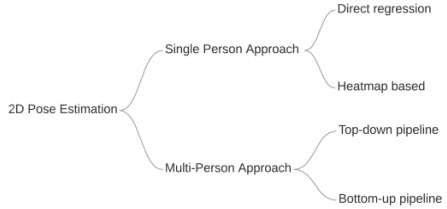
\includegraphics[scale=1]{gambar/taxonomy-pose-estimation.png}

  % Ubah dengan keterangan gambar yang diinginkan
  \caption{Taxonomy of pose estimation approaches}
  \label{fig:pose-estimation}
\end{figure}

Pose estimation is a heavily explored area with applications in gaming, animation, action recognition, activity tracking, and augmented reality.
In order to improve pose estimate outcomes, various approaches have been developed. These methods may generally be split into: Single-person and Multi-person approaches, 
as depicted in figure \ref{fig:pose-estimation}. The single-person approach is fundamentally a regression issue because it just determines the pose of a single person in an image, 
the person's position and an implicit number of keypoints are already known. However, the multi-person approach tries to solve an unconstrained problem because we do not know 
the positions and number of persons within the image \parencite{romeo}.

The single-person approach is divided into two frameworks based on the keypoint prediction method: directly regressing keypoints from the features (i.e. direct regression based framework)
or by generating heatmaps and inferencing keypoints via heatmap (i.e. heatmap based framework) \parencite{romeo}.
A direct regression-based framework can be implemented in various ways: as done by \parencite{toshev2014}, 
they presented DeepPose where their model uses a simple architecture with a convolutional layer, followed by a dense layer that will produce keypoint values in \emph{(x,y)}.
Other authors \parencite{carreira2015} suggested a technique that iteratively improves model output by feeding back mistake predictions, leading to a notable improvement in accuracy.

Then for a heatmap based framework, an alternative method can be used to generate heatmaps of all keypoints in the image
rather than directly predicting them. The final stick figure is then created using additional techniques to know the connection between keypoints or joints.
In \parencite{chen2014}, authors proposed a graphical model with pairwise
relations to make adaptive use of local image measurements. Later on, both the detection of joints and the prediction of their relationships can be accomplished using those local image measurements.
\parencite{newell2016} designed a \emph{"stacked hourglass"} network, that is closely similar to encoder-decoder architecture and is based on the sequential phases of pooling and upsampling.
They demonstrated the importance of repeated bottom-up, top-down processing with intermediate supervision for enhancing the effectiveness of human pose detection.

The multi-person approach is a more complex task because
the positions and number of persons within the image are unknown, therefore the framework has to detect keypoints and assemble an unknown number of persons. To overcome this task,
two pipelines have been proposed: top-down pipeline and bottom-up pipeline \parencite{romeo}.
Beginning with the detection of every person present in an image, the top-down pipeline creates bounding boxes. The following action uses each of the identified bounding boxes and applies a single-person method. 
For each person that is discovered, the single-person technique will generate keypoints, and then, as shown in Figure \ref{fig:top-down-approach}, the pipeline may include extra steps of post-processing and improving final results.

\begin{figure}[ht]
  \centering
  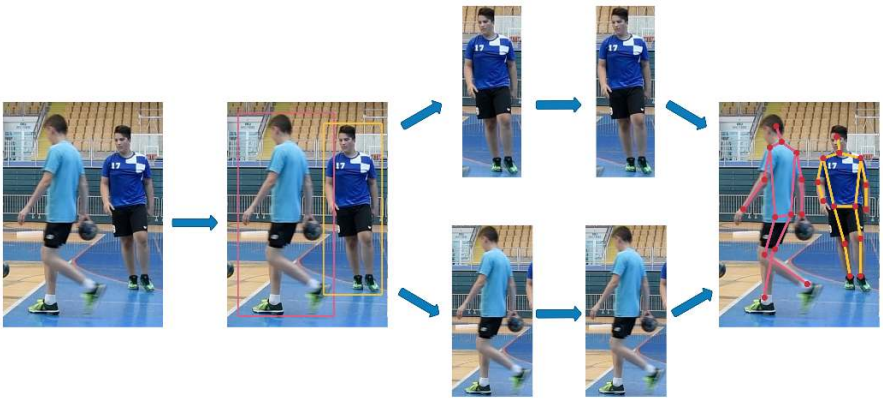
\includegraphics[scale=0.8]{gambar/top-down-approach.png}
  \caption{The top-down pipeline in multi-person approach for pose estimation}
  \label{fig:top-down-approach}
\end{figure}

Compare to a top-down pipeline, the bottom-up pipeline operates in reverse. The bottom-up pipeline begins by finding all of the keypoints, which are then connected to human instances, as seen in Figure \ref{fig:bottom-up-approach}. 
The bottom-up pipeline is probably quicker than the top-down pipeline because it doesn't detect human bounding boxes and runs pose estimation for each person individually.

\begin{figure}[ht]
  \centering
  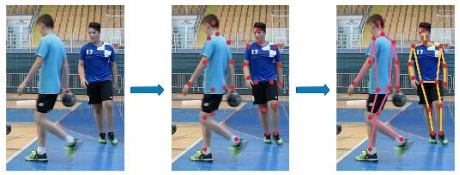
\includegraphics[scale=1.2]{gambar/bottom-up-approach.png}
  \caption{The bottom-up pipeline in multi-person approach for pose estimation.}
  \label{fig:bottom-up-approach}
\end{figure}

\section{Human Pose Estimation}
\label{sec:humanposeestimation}

Estimating human poses is one of the most challenging things in computer vision, which aims to determine the position or spatial location of certain points of a person's body (body parts/joints) from a given image or video.
Essentially it is a way to capture a set of coordinates by defining the human body joints like wrist, shoulder, knees, eyes, ears, ankles, and arms, which is a key point in images and videos that can describe a pose of a person. Then, when an image or video is given to the pose estimator model as input, it identifies the coordinates of these detected body parts and joints as output and a confidence score showing the precision of the estimations.
For many years, the main topic of discussion for numerous classical object detection applications has been the detection of persons.
With recent developments in machine-learning algorithms, computers can now understand human body language by performing pose detection and pose tracking. It has now reached a point where the hardware requirements to operate and the detection accuracy make them commercially viable.
Several industries, including security, business intelligence, health and safety, and entertainment, will be profoundly impacted by human pose estimate. Autonomous driving is one such application where this method has already shown its viability. Computers can sense and predict pedestrian behavior far more comprehensively with the use of real-time human pose detection and tracking, allowing for more consistent driving.

Pose estimation on humans can be divided into two techniques: 2D Pose Estimation and 3D Pose Estimation.
2D pose estimation is a type of pose estimation that can estimate the locations of the body joints in 2D space relative to input data (i.e., image or video frame). The location is represented with X and Y coordinates for each key point. On the other hand, 3D pose estimation transforms a 2D image into a 3D object by estimating an additional Z-dimension to the prediction. 3D pose estimation enables us to predict the accurate spatial positioning of a represented person or thing.

In the early days, the pose estimation job was treated as a part-based inference task, and there were two general groups of models. The first one is called appearance models, where features of body parts are first extracted by feature descriptors like Histogram of Oriented Gradient then distinct body parts are combined together.
Another group of models is deformable models or structural models. 
The performance of estimation models rapidly increases after deep convolutional networks are used for pose estimation. Researchers initially concentrate primarily on a well-cropped single-person posture estimate problem, which is a simplified sub-task. These days, more difficult situations, including pose estimation in a crowd, have become hot subjects thanks to the success of the more general multi-person pose estimation \parencite{song2021}.

\section{Humanoid Robot Pose Estimation}
\label{sec:humanoidrobotposeestimation}

Humanoid robots and people have similar shapes, which has both advantages and disadvantages. On the one hand, this allows us to start with approaches already in use for people, but on the other, it makes it harder for us to distinguish between people and humanoid robots \parencite{amini2021}.
as explained in Section \ref{sec:poseestimation}, in general, the effort to tackle the problem of pose estimation is vary depend on the number of persons (single-person or multi-person), for multiple persons can be categorized as a top-down or bottom-up approach.
In the top-down approach, the initial stage is to identify specific individuals, and the subsequent step is to implement pose estimation. The fact that the model's performance is closely associated with the performance of the person detector is one of the drawbacks of this approach. Although the state-of-the-art (SOTA) results are derived from this type of approach,  the runtime of such approaches is negatively affected by the number of persons present,
as a single-person pose estimator is run for each detection. Since the computational cost grows linearly as the number of users increases, performance is frequently not real-time \parencite{amini2021}.

Bottom-up techniques, on the other hand, are less reliant on the number of people in the image because they simultaneously identify body joints and classify them into individuals. Accurately grouping the detected keypoints in real-time is one of the bottom-up method's fundamental issues.
Recent methods arrange the identified keypoints into distinct instances using a greedy algorithm. In addition, compared to the top-down method, the bottom-up method's effectiveness is more influenced by the various scales of the people in a given image. Previous research has relied on high-resolution input size \parencite{papandreou2018} or the scale search method \parencite{cao2019} to address this issue. However, the inference time is growing as a result of these strategies.
A time-efficient method predicting keypoints at higher resolution was introduced by Cheng et al. \parencite{cheng2020}, narrowing the performance gap between bottom-up and top-down models.

There are three Pose Estimation Models for humanoid robots that we retrained with the
new dataset. All of them used bottom-up approaches. For a detailed explanation of each model is located in following section.

\subsection{NimbRo's Model}
\label{subsec:nimbromodel}

NimbRo's model chose to use a similar architecture with NimbRo-Net and NimbRo-Net2 because it had such positive outcomes. Their model is an single-stage encoder-decoder network which takes an RGB image of
size \emph{w x h}. The model predicts heatmaps of both keypoints and limbs for scale 1/4 and only
heatmaps of keypoints for scale 1/2, where each scale is supervised with an intermediate loss \parencite{amini2021}. The full network architecture is depicted in Figure \ref{fig:nimbro-model-architecture}.

\begin{figure}[ht]
  \centering
  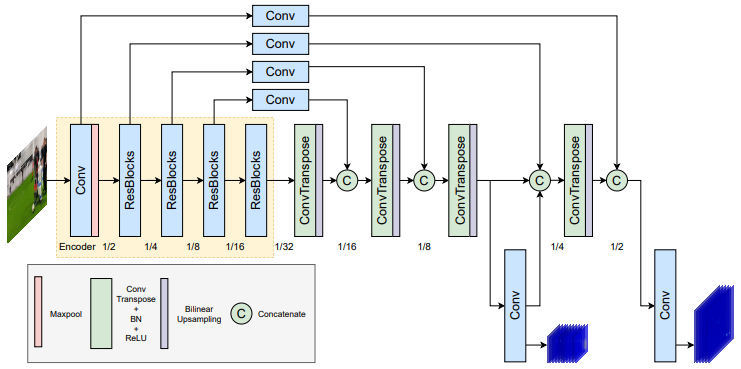
\includegraphics[scale=0.9]{gambar/nimbro-architecture.png}
  \caption{NimbRo's model architecture}
  \label{fig:nimbro-model-architecture}
\end{figure}

\subsection{YOLO-pose}
\label{subsec:yolopose}

Although this architecture is intended for humans, but it may be used for humanoid robot too, as explained in Section \ref{sec:humanoidrobotposeestimation}.
YOLO-pose is a single-shot approach like other bottom-up approaches. However, it doesn't use heatmaps. Rather, it associates all keypoints of a person with anchors. It is
based on YOLOv5 object detection framework and can be extended to other frameworks as well. Figure \ref{fig:YOLO-pose-architecture} illustrates the overall architecture with keypoint
heads for pose estimation. The Input image is passed through darknetcsp backbone that generates feature maps at
various scales {P3, P4, P5, P6}. PAnet is used for fusing these feature maps across multiple scales and the output is fed to detection
heads. Finally each detection head branches into box head and keypoint head \parencite{maji2022yolopose}.

\begin{figure}[ht]
  \centering
  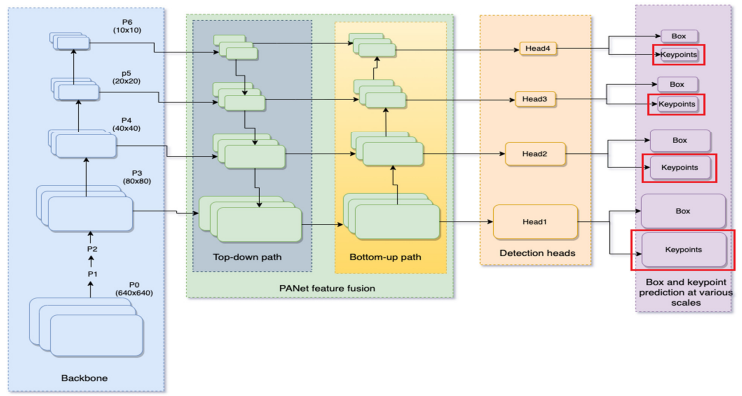
\includegraphics[scale=1]{gambar/yolo-architecture.png}
  \caption{YOLO-pose architecture.}
  \label{fig:YOLO-pose-architecture}
\end{figure}

\subsection{RCNN}
\label{subsec:rcnn}
\cleardoublepage

% Bab 3 desain dan implementasi
\chapter{DESIGN AND IMPLEMENTATION}
\label{chap:desainandimplementation}

% Ubah bagian-bagian berikut dengan isi dari desain dan implementasi

This chapter describes the design and implementation of the system that has been created.
As seen in Figure \ref{fig:block-diagram}, there are 2 main block diagrams. The left one is a block diagram for RECORD mode and the right one is for PLAY mode.
In RECORD mode, it starts with a human image and then does pose estimation to get human keypoints. After that, we convert the angle between 2 keypoints into a servo value so we can move the robot's servo to mimic human movement and save it for PLAY mode.
On the other hand, in PLAY mode, the input is 2: human image and humanoid robot image. Then, we perform pose estimation for both images. Before doing keypoint normalization, we have to choose 6 human keypoints based on humanoid robot keypoints. Lastly, we compare those keypoints and get the result.
\begin{figure}[ht]
  \centering
  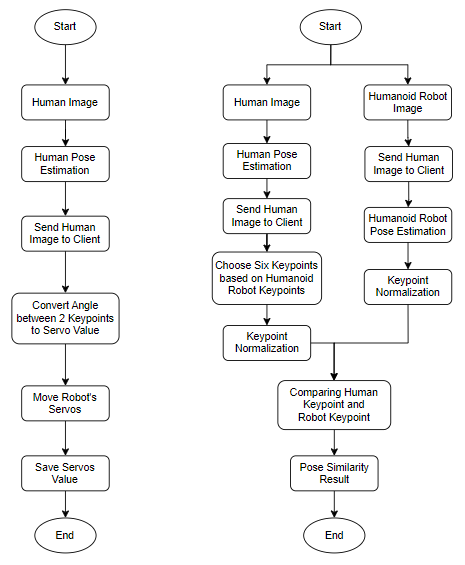
\includegraphics[scale=1.23]{gambar/diagram-block-revisi.png}
  \caption{Block Diagram of Workflow.}
  \label{fig:block-diagram}
\end{figure}
In the section that follows, each block is explained in further depth. Note that maybe there is a merge explanation if we use the same technique for different blocks. For instance, a block that sends a human image to the client and the block that send a robot image to the client will be merged to become just send an image to the client.


\section{Input Image}
\label{sec:input-image}

The input image that is fed into both models (human and humanoid robot) is 640x480 pixels with RGB channels. The device for getting the image is the Logitech C920 Webcam. We use OpenCV library to open the camera and capture the image.


\section{Human Pose Estimation}
\label{sec:human-pose-estimation}

Since there are already many pose estimation models for humans out there, we do not need to retrain them and just compare them to find the best model. In order to compare the models, we selected a paper for reference.
So evaluation metrics based on paper and real detection results will be shown in Chapter \ref{chap:resultsandiscussion} but for inference time, we will try in NUC i5. The models that we compare include OpenPose, MediaPipe, and YOLO-pose.
The input for these models is an RGB image and the output is the location of human keypoints.


\section{Send Image to Client}
\label{sec:send-image-to-client}

Our main program uses websites to interact with users because of its flexibility on any platform, the website view can be seen in Figure \ref{fig:websiteview}. So there is a Javascript client and a Python Server that communicate via \emph{socketio}.
The server will send human image to the client so we can adjust our position in the camera. This is done to enable the robot to capture the entire human pose.
\begin{figure}[ht]
  \centering
  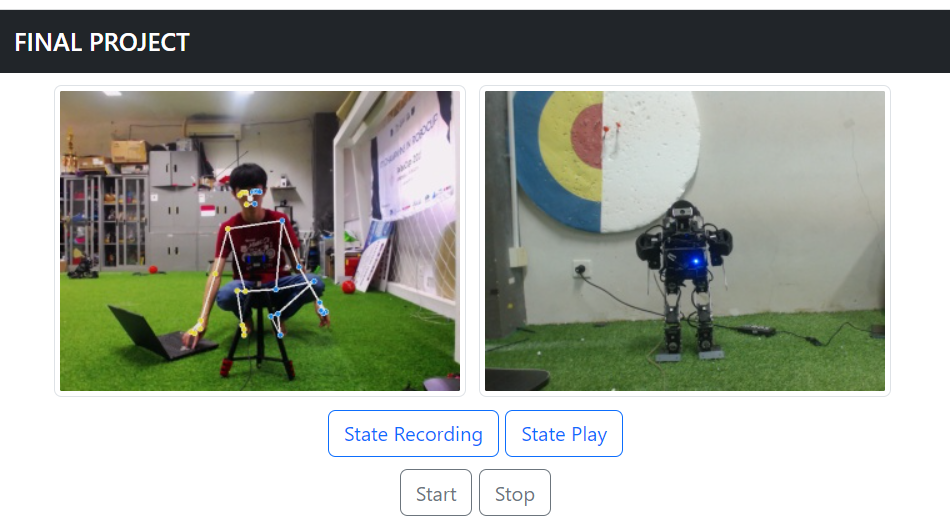
\includegraphics[scale=0.7]{gambar/web.png}
  \caption{Website View.}
  \label{fig:websiteview}
\end{figure}
The main program is divided into two modes, RECORD mode and PLAY mode. In RECORD mode, a human as a trainer gives a series of movements and will be followed by a humanoid robot, as well as robot saves these movements to use in PLAY mode later.
Meanwhile, in the PLAY mode, the robot acts as a trainer and performs a series of movements according to the movements previously stored in RECORD mode. Human will follow the robot's movement while the robot is also saving both human and robot images and comparing them later.

After getting human's keypoint, the server will visualize the detection result and send it as a buffer to the client.
On the client side, we use ReactJS library. There are four buttons: RECORD, PLAY, START, and STOP button. The RECORD and PLAY button indicates the modes in the main program, while the START and STOP button tell us when the mode is started or stopped.
There is a different color after we click on a button to indicate that we have pressed that button.
Apart from that, there are also two images that show human and robot image, actually in RECORD mode there is only one image (human image), while in PLAY mode there are 2 images (human and robot image). 
In our program, we define that client and server communicate through port 5555, where server can send image to client and client can send some data back to the server like current mode and time to start or stop the mode.
We use the \emph{useEffect} function to indicate if there is a change in a particular variable and do something like converting the image from the buffer to a string in order to display it on the HTML image tag.


\section{Convert Angle to Servo Value}
\label{sec:convert-angle-to-servo-value}

This section and Section \ref{sec:move-robot-servo} are triggered when the button RECORD and START is pressed on the website, so the client sends this information to the server and it does the calculation. 
To be able to move a robot's upper body like human movement, we need to obtain the angle between 2 keypoint using the \emph{arc tangent} function with the input \emph{\{x,y\}} keypoint coordinate.
Since we use MediaPipe Pose to detect human keypoints based on the result and discussion in Section \ref{sec:humanmodelcomparison}, the output is a normalized point, so we multiplied the x and y coordinates with the width and height image respectively to get the real pixel value.
Afterward, we subtract the second y keypoint value with the first y keypoint value and divided it by the second x keypoint value subtract with the first x keypoint value, and input the result to the \emph{arc tangent} function, as shown in Equation \ref{eq:arctan}.
\begin{equation}
  \label{eq:arctan}
  angle = \arctan \left(\frac{Y_2 - Y_1}{X_2 - X_1}\right)
\end{equation}

There are four angles we want to retrieve which are the angles from the shoulder to the elbow (right and left) and also the elbow to wrist (right and left) in order to robot can mimic upper body human movement.
If we look at MediaPipe Pose Landmark in Figure \ref{fig:mediapipe-landmark}, 6 keypoints that become our concern are 11, 12 for shoulders, 13, 14 for elbows, 15, and 16 for wrists. 
We get the right shoulder values by entering landmark 14 as the second argument and landmark 12 as the first argument of the \emph{arc tangent} function. This also applies to get the left shoulder angle value by entering landmarks 13 and 11 respectively. 
It is slightly different to obtain the elbow angles because we want its angle to be relative to the shoulder angle by subtracting its angle from the shoulder angle. We also apply limitations for each angle to keep the servo safe and not hit the robot body or other servo as seen in Table \ref{tb:robot-servos}.

\begin{longtable}{ccc}
  \caption{Robot Servos Limitations.}
  \label{tb:robot-servos}\\
  \hline
  \rowcolor[HTML]{C0C0C0}
  \textbf{Joint Angle} & \textbf{Motion} & \textbf{Range (deg)} \\
  \hline
  LShoulderPitch       & Left shoulder joint right and left    & -110 to 30  \\
  RShoulderPitch       & Right shoulder joint right and left   & -30 to 110 \\
  \rowcolor[HTML]{C0C0C0}
  \textbf{Joint Angle} & \textbf{Motion} & \textbf{Range (deg)} \\
  \hline
  LElbowRoll           & Left Elbow joint front and back       & -120 to 10  \\
  RElbowRoll           & Left Elbow joint front and back       & -10 to 120  \\
  \hline
\end{longtable}


\section{Move Robot's Servos}
\label{sec:move-robot-servo}

The program to move the robot's servos takes the same place as the program for the server. Our main program uses ROS2 with Python language. To be able to run the server and ROS2 program simultaneously, we need a separate thread, so the server program does not block the ROS2.
In the ROS2 framework, every package has its own functionality. On this occasion, we divide the task to move the robot's servo into 2 packages. The first one is named \emph{motion matching} where the server program and angle conversion to servo value happen, the other one is \emph{tachimawari},
a package that provides a DYNAMIXEL's joints management library for a ROS 2 project. This package name comes from a Japanese word that means motion. Every package has a node with the package's name like Figure \ref{fig:relation-node-record-mode}.
We can see this node relationship from rqt graph or ROS2 client interfaces, but we choose rqt graph because it is more visual.
\begin{figure}[ht]
  \centering
  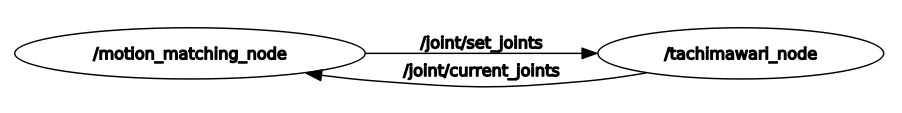
\includegraphics[scale=0.62]{gambar/rqt_without_akushon.png}
  \caption{Relationship Between Nodes in RECORD Mode.}
  \label{fig:relation-node-record-mode}
\end{figure}

Each node communicates with each other through a topic. There are 2 topics in RECORD mode, which are \verb|joint/set_joints| and \verb|joint/current_joints|. 
After getting desired servos angle from the previous section, we just need to publish it to \emph{tachimawari} node and it will move the servos. In the \emph{motion matching} node, there is a publisher that publishes servos angle to \verb|joint/set_joints| topic after the detection process and calculation is done, and also a subscriber in \emph{tachimawari} node that subscribes
to the same topic which collects the data that is published from the publisher. \verb|joint/set_joints| topic uses an interface like code snippet \ref{lst:set-joint-msg}, where there are \verb|control_type| variable with type integer and an array with Joint type, each joint consist of id and position like code snippet \ref{lst:joint-msg}.
\begin{lstlisting}[
  language={},
  caption={Joint msg.},
  label={lst:joint-msg}
]
uint8 id
float32 position
\end{lstlisting}

\begin{lstlisting}[
  language={},
  caption={SetJoints msg.},
  label={lst:set-joint-msg}
]
int8 control_type 4
Joint[] joints
\end{lstlisting}

In \verb|tachimawari_node| there is \verb|joint_node| that publishes the current joints every 8ms (it is used in the following section) and has a subscriber that listens to joints that we want to move. 
In order to move servos to the value that we want, we must enable the torque of all servos first. Then we make a command in array form that contains the servo's id and our desired value or target value (16 bytes) that split into 2 * 8 bytes.
For example, our target value is 512 (in binary is equal to \verb|00000010 00000000|), and the message that we send is 2 (\verb|00000010|) and 0 (\verb|00000000|). We can acquire that by performing bitwise AND and bitwise right shift. The bitwise AND operation is performed between the target value and \verb|0xFF|, which is represented as \verb|00000000 11111111| in binary.
Since \verb|0xFF| has 0 bits in the higher byte and 1 bits in the lower byte, the result of the operation is the lower byte of the target value. On the other hand, the bitwise right shift operator is used to shift the bits of the target servo 8 positions to the right. Shifting the bits to the right by 8 positions effectively discards the lower byte, leaving only the higher byte in the result.
It is the same when we receive the present position from the servo, the servo also sends the data in two bytes (lower and higher) and we need to combine the lower and higher bytes to reconstruct the 16-bit value representing the present position. This can be achieved by performing a left shift operation on the higher byte. Shifting it 8 bits to the left effectively moves it to the higher-order byte position.
After that, the bitwise OR operator combines the shifted higher byte with the lower byte. This operation merges the two bytes to form a 16-bit value representing the present position.


\section{Save Servos Value}
\label{sec:save-servo-value}

In the previous section, we discussed a little about the publisher in \emph{tachimawari} package that publishes the value of every current joint of the robot through a \verb|joint/current_joints| topic.
There is also a subscriber in \verb|motion_matching| node that is retrieved that data and a ROS2 timer that is triggered every 0.5 seconds to save the current joints in a JSON format like code snippet \ref{lst:json-save-joints} so our robot can move according to the movements exemplified by humans. 
The provided JSON format represents a structured data object that describes a specific action or movement sequence. There is "poses" array contains multiple pose objects, each representing a particular joint configuration during the action.
Each pose object includes a "joints" sub-object, which lists different joints and their corresponding values. For example, \verb|"left_ankle_pitch"| has a value of 25, \verb|"left_ankle_roll"| is set to 0, and so on. These values represent the positions or angles of the respective joints.
Each pose object also has a "name" field to identify the pose. The "pause" field specifies the duration of the pause between this pose and the next one, while the "speed" field indicates how fast this pose will be executed.
Lastly, the \verb|"start_delay"| field denotes any delay before the action begins, and the \verb|"stop_delay"| field signifies the delay after the action finishes before the robot stops. In total, there are 20 servos in our robot, so in the actual JSON file each "joint" sub-object has 20 items with their respective joint names.

\begin{lstlisting}[
  language={},
  caption={JSON Format to Save Joints Value.},
  label={lst:json-save-joints}
]

  "poses": [
    {
      "joints": {
        "left_ankle_pitch": 25,
        "left_ankle_roll": 0,
        ...
      },
      "name": "pose name",
      "pause": 0,
      "speed": 0.003
    },
  ],
  "start_delay": 0,
  "stop_delay": 0

\end{lstlisting}


\section{Humanoid Robot Pose Estimation}
\label{sec:humanoid-robot-pose-estimation}

This explanation is intended for the right block diagram from Figure \ref{fig:block-diagram} or we can also say as the RECORD mode. The difference between the PLAY and RECORD modes lies in the number of cameras used.
So there will be two cameras, one camera to record human movement (located on the robot's head) and the other to record robot movement (located from the human side facing the robot), the distance between them approximately 1 - 1.5 meters, as shown in Figure \ref{fig:pose-comparison-side}.
In PLAY mode, the server side sends two images so that we can know and adjust the position of humans and robots in the camera. Due to the large network delay when sending two 320x240 pixel images, when the START button is pressed,
the server does not send the image to client again, the robot plays a series of moves stored in the previous JSON file by communicating via another ROS2 packages, while saving both images. After that, when the STOP button is pressed, the server starts to compare poses between them.
\begin{figure}[ht]
  \centering
  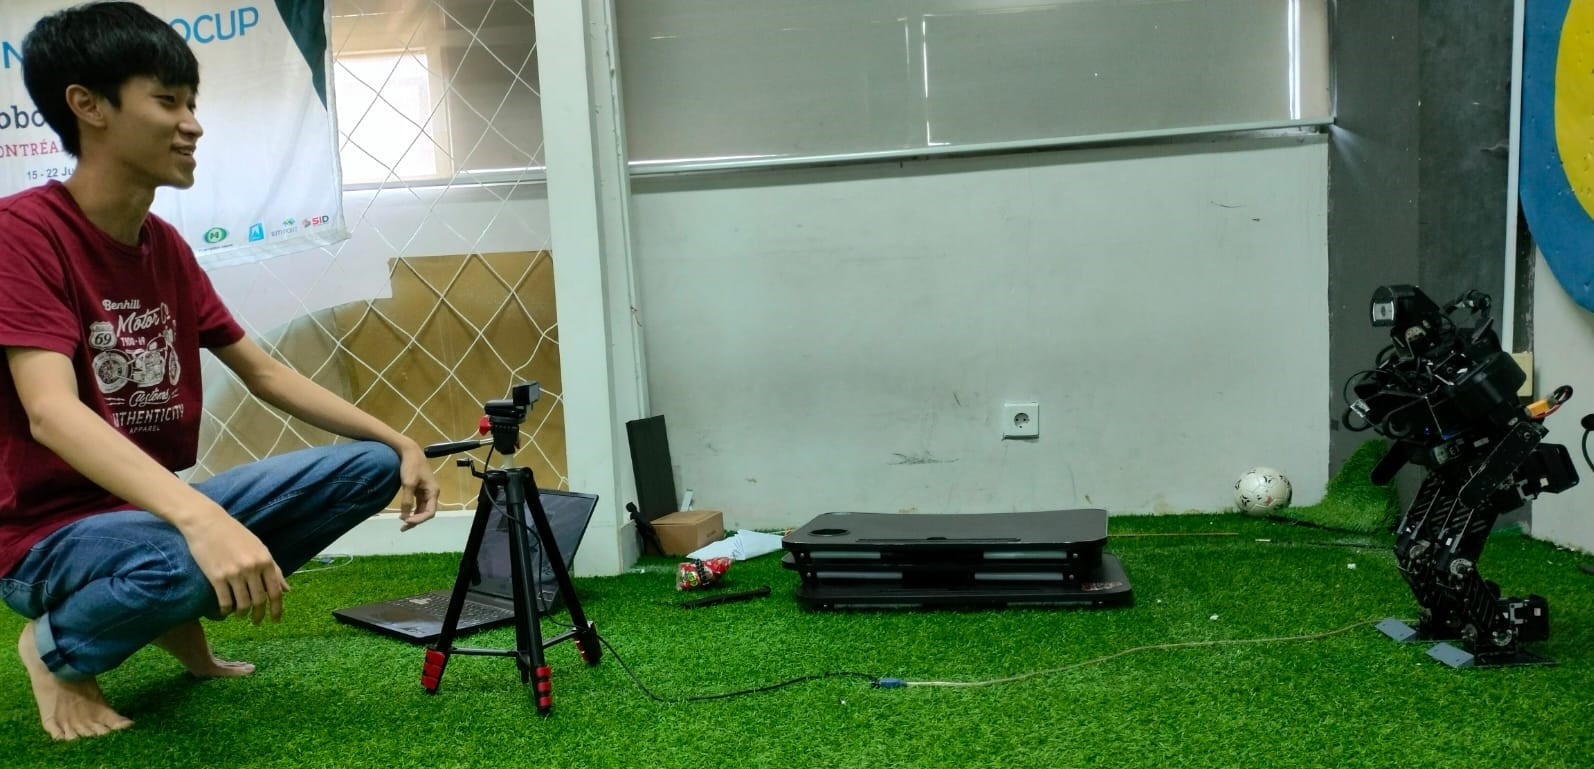
\includegraphics[scale=0.3]{gambar/pose-comparison.jpeg}
  \caption{Pose Comparison from Side.}
  \label{fig:pose-comparison-side}
\end{figure}

In order to move the servo robot according to the data stored in JSON, a package called \emph{akushon} is needed. \emph{Akushon} is a package related to motion robots. This package name comes from a Japanese word that means action.
Like Section \ref{sec:move-robot-servo}, every package has a node with the package's name and communicates with each other through a topic as shown in Figure \ref{fig:relation-node-play-mode}. There are 3 topics in PLAY mode: \verb|joint/set_joints|, \verb|joint/current_joints| that is used between \verb|akushon_node| and \verb|tachimawari_node| also \verb|motion_matching_node| and \verb|tachimawari_node|,
and \verb|action/run_action| that is used between \verb|akushon_node| and \verb|mo| \verb|tion_matching_node|.
The explanation about how to move the robot's servos and get the current value of servos through topic \verb|joint/set_joints| and \verb|joint/current_joints| is located in Section \ref{sec:move-robot-servo}.
Meanwhile, topic \verb|action/run_action| is used to send pose data in a JSON file from \emph{motion matching} to \emph{akushon} package. In \emph{akushon} package there is an interpolator that loops through every pose in the JSON file, get every value of the servo, and send it to \emph{tachimawari} package.
\begin{figure}[ht]
  \centering
  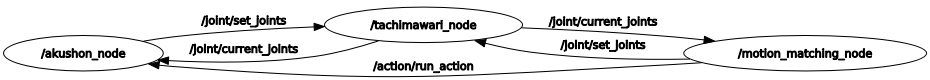
\includegraphics[scale=0.64]{gambar/rqt_akushon.png}
  \caption{Relationship Between Nodes in PLAY Mode.}
  \label{fig:relation-node-play-mode}
\end{figure}

This section immediately begins with the estimation pose for humanoid robot because the explanation regarding the previous block has been explained in the previous section.
Since there are not many pose estimation models for humanoid robots out there yet, we need to retrain them or use transfer learning from the model that supposes to estimate human pose.
Therefore, the first step is making a new humanoid robot pose dataset.

\subsection{Make New Dataset}
\label{subsec:make-new-dataset}

This new dataset is a merge of NimbRo's Humanoid Robot Pose dataset and Ichiro's dataset. NimbRo's dataset contains both single and multiple robots to
simulate RoboCup's real conditions. They also gathered from RoboCup Humanoid League YouTube videos, their own internal videos, and ROS bags. 
Overall, their dataset has over 1.5k images that come from 23 videos with around 2.3k robot instances. These images include teen and adult-sized robots and contain more than ten different robot types \parencite{amini2021}.
However, the robots in Ichiro's dataset are only kid-sized and come in single or maximum two-robot configurations. The images in our dataset come from videos that are taken in our lab. 
Then we split up those videos into multiple images and we pick not blurred videos.
Before merging, we need to fix NimbRo's dataset format first. This is because after we visualized some of their data, we found that the bounding boxes in \emph{annotations} part were misplaced (the width and height were swapped).
After we refine their dataset format and merge them with our dataset, the newly created dataset has approximately 2.1k images.
About 20 percent of the dataset was used for scoring and validating.

When it comes to annotation tools, there are a lot of choices out there including offline and online tools. We have tried some of them like Dataloop, V7labs, or Supervisely which is recommended by NimbRo.
However, when we tried to export the dataset into COCO format, it failed (e.g. can not import it or it can be imported but the JSON result in the annotation section is none). So, we decided to use a coco-annotator,
a web-based image annotation tool designed for versatility and efficiently labeling images to create training data. Regarding the number of keypoints in each robot, we followed NimbRo's dataset.
There are six keypoints including head, trunk, hands, and feet. We stick to that idea because we want to try the model's performance and inference time with fewer keypoints first and if we are confident enough, we will increase the number of keypoints later.

\subsection{Training Pose Estimation Model for Humanoid Robot}
\label{subsec:training-robot}

All of the training processes in this study were primarily conducted on a DGX-A100 server computer and written in the Python programing language. The specific configuration explains in Table \ref{tb:dgxa100}.
From this base specification, we are allocated a Jupiter notebook container with
python and many libraries preinstalled with following allocated resources explained in Table \ref{tb:allocatedcontainer}.
\begin{longtable}{|c|c|}
  \caption{DGX-A100 Specification.}
  \label{tb:dgxa100}\\
  \hline
  CPU     & Dual AMD Rome 7742, 128 cores total @ 2.25 GHz \\
  \hline
  GPU     & 8 x NVIDIA A100 80 GB Tensor Core GPUs  \\
  \hline
  RAM     & 2 TB \\
  \hline
  Storage & 30 TB (8 x 3.84 TB) U.2 NVMe drives \\
  \hline
\end{longtable}

\begin{longtable}{|c|c|}
  \caption{Allocated container specification.}
  \label{tb:allocatedcontainer}\\
  \hline
  GPU     & 1/8 NVIDIA A100 GPU \\
  \hline
  GPU RAM & 10 GB  \\
  \hline
  CPU RAM & 8 GB \\
  \hline
  Storage & 100 GB  \\
  \hline
\end{longtable}

\subsubsection{NimbRo's Model}
\label{subsubsec:training-nimbro-model}

The hyperparameters that are used to train NimbRo's model followed the description in their paper.
This model is trained using the AdamW optimizer with a learning rate of 10\textsuperscript{-4},
batch size 16, and weight decay of 10\textsuperscript{-4} for the total 200 epochs.
Note that the encoder is initialized by pre-trained ResNet weights on ImageNet.
We also use data augmentation that includes random scaling and random translation during training \parencite{amini2021}.
We do not use random horizontal flip and random rotation like NimbRo did because in our case it will make the training result worse.

The main program for training is already made by them named \emph{main.py} using PyTorch framework, we just need to run it on Jupyter Notebook file or Terminal and adjust the arguments for our needs.
In their script, there is an argument name \verb|config| which it is referred to a file where we store all the hyperparameters, number of epochs, dataset name for training and testing, and many others. 
Another argument tells us about a directory path where we save training results and the dataset takes place.
\lstinputlisting[
  language={},
  caption={Example YAML file config for NimbRo's Training.},
  label={lst:confignimbro}
]{files/train_nimbro.yaml}
File \ref{lst:confignimbro} is an example of YAML configuration file for NimbRo Training. This is not a complete version, but we included parts that were changed frequently during the training process.
The "SEED" is set to 42, ensuring reproducibility of random processes. The "DEVICE" is specified as "cuda", indicating the utilization of a GPU for computation.
\verb|"BATCH_SIZE"| is set to 16, meaning that 16 data samples will be processed together in each training iteration. If we make \emph{batch size} value larger, it requires more memory to store the input data, intermediate activations, and gradients during training.
If the available memory is limited, increasing the batch size beyond the memory capacity may lead to out-of-memory errors or cause the training process to slow down.
However, larger batch sizes can speed up the training process as more samples are processed in parallel. It also effect the generalization capability of the model.
Smaller batch sizes tend to provide more stochasticity during training, which can act as a form of regularization and help prevent overfitting. In contrast, larger batch sizes may result in a smoother optimization process, potentially leading to faster convergence but with a slightly increased risk of overfitting.
The \verb|"NUM_WORKERS"| is set to 2, indicating that two worker processes will be used to load and preprocess the data.

The training process will run for 200 epochs as specified by \verb|"NUM_EPOCHS"|. When training for more epochs, the model undergoes more iterations and updates, allowing it to refine its learned representations and adjust its parameters based on the training data.
This can lead to improved model performance as the model converges towards an optimal solution and achieves higher accuracy on both the training and validation data. However, it is important to be cautious of the risk of overfitting. Overfitting occurs when the model becomes too specialized to the training data and fails to generalize well to unseen data.
Increasing the number of epochs without proper regularization techniques can increase this risk. The model may start to memorize the training data instead of learning generalizable patterns, resulting in poor performance on new data. Additionally, training for a greater number of epochs requires more time.
The \verb|"PRINT_FREQ"| is set to 100, meaning that training progress and relevant information will be printed or displayed every 100 iterations.

The "DATASET" section contains settings related to the dataset used for training.
The \verb|"DATASET.TRAIN"| specifies the name or identifier of the training dataset folder, and \verb|"DATASET| \verb|.TEST"| indicates the name of the validation dataset folder. The \verb|"NUM_KEYPOINTS"| is set to 6, denoting the number of keypoints or landmarks in the dataset, while \verb|"NUM_LIMBS"| is set to 5, representing the number of limbs or connections between keypoints.
The \verb|"MAX_NUM_| \verb|DETECTIONS"| is set to 10, indicating the maximum number of robots in the dataset. The "SIGMA" parameter is set to 2.0, which is used in generating heatmaps. For augmentation, The "FLIP" is set to 0.0, meaning there will be no horizontal flipping of the input data. The "TRANSLATE" is set to 0.4, allowing the data to be translated by up to 40\% of its size.
The "SCALE" parameter represents a range of scaling applied to the input data, with a minimum scale of 0.5 and a maximum scale of 1.5. The "ROTATION" is set to 0, indicating no rotation will be applied to the input data. Additionally, the \verb|"INPUT_SIZE"| is set to [384, 384], representing the desired input size of the model, while the \verb|"OUTPUT_SIZE"| is set to [192, 192], indicating the desired output size.

For computing loss, they use mean square error (MSE) between the predicted heatmaps and the ground truth heatmaps for both keypoints and the limbs.
This loss function directly compare the predicted coordinates of the keypoints with the ground truth coordinates by averaging the squared difference between the predicted and target coordinates.
Finally, the total loss used to train the network is the sum of the keypoint loss and the limb loss \parencite{amini2021}.

\subsubsection{YOLO-pose}
\label{subsubsec:training-yolo-pose}

Before we jumped into training process, we must change format of our newly dataset from COCO to YOLO. Differ from COCO format, YOLO format gives keypoint confidence or visibility flag 2 for either visible or occluded keypoint
and if it is outside the field of view, the value is set to zero. However, COCO format defines visibility flag as v=0: not labeled, v=1: labeled but not visible, and v=2: labeled and visible. So, we change the definition of
v=1 and v=2 become just v=2 in YOLO format and keep v=0. As seen in Pseudocode \ref{lst:change-keypoint-format}, where we make a function called \verb|change_keypoint_format| which has 2 input arguments and return new keypoints with YOLO format. 
Beside keypoint format differences, bounding-box format between them is also different. COCO defines a bounding-box as follow: x (top left), y (top left), width, and height. On the other hand,
bounding-box format in YOLO is: x (center), y (center), width, and height also all of them need to be normalized. Thus, we need to add 1/2 width to x, 1/2 height to y like in Pseudocode \ref{lst:change-bbox-format}, and normalize them by multiplying new x and y with 1/width and 1/height respectively. 

\lstinputlisting[
  language={},
  caption={Change Keypoint Format From COCO to YOLO.},
  label={lst:change-keypoint-format}
]{program/change-keypoint.txt}

\lstinputlisting[
  language={},
  caption={Change Bounding Box Format From COCO to YOLO.},
  label={lst:change-bbox-format}
]{program/bbox-norm.txt}

The hyperparameters to train YOLO-pose followed the description in their GitHub named \emph{hyp.pose.yaml}.
We use SGD optimizer with a cosine scheduler. The base learning rate is set to 10\textsuperscript{-2}, batch size 16,
and weight decay of 5\textsuperscript{-4} for total 150 epochs. There are also data augmentation like random scale ([0.5, 1.5]),
random translation [-10, 10], mosaic augmentation with probability 1, and various color augmentations.
It is the same with previous section, the main program for training has been provided using PyTorch framework too, but the program is intended for humans with 17 keypoints.
If we run it directly with our dataset with 6 keypoints, an error will be raised. Therefore, a little bit of code needs to be changed to make the training process can be run.

The overall loss for YOLO-pose is a sum of loss for classification, bounding box, keypoints, and keypoints confidence with its threshold as seen in Equation \ref{eq:overall-loss-yolo}.
The hyper-params that are chosen to balance between losses at different scales are $\lambda_{cls} = 0.5$, $\lambda_{box} = 0.05$, $\lambda_{kpts} = 0.1$, and $\lambda_{kpts_conf} = 0.5$.
Note that, Loss at location (\emph{i,j}) is valid for k\textsuperscript{th} anchor at scale s if a ground truth bounding box is matched against that anchor \parencite{maji2022yolopose}.
\begin{equation}
  \label{eq:overall-loss-yolo}
  \mathcal{L}_{total} = \sum_{s,i,j,k} (\lambda_{cls}\mathcal{L}_{cls} + \lambda_{box}\mathcal{L}_{box} + \lambda_{kpts}\mathcal{L}_{kpts} + \lambda_{kpts_conf}\mathcal{L}_{kpts_conf})
\end{equation}

Instead of using distance-based loss for box detection, the majority of modern object detectors optimize advanced IoU loss variants like GIoU, DIoU, or CIoU loss since these losses are scale-invariant and directly optimize the evaluation measure itself.
They use CIoU loss for bounding box supervision. For a ground truth bounding box that is matched with k\textsuperscript{th} anchor at location (\emph{i,j}) and scale s, loss defined as follows \parencite{maji2022yolopose}.
\begin{equation}
  \label{eq:bbox-loss-yolo}
  \mathcal{L}_{box}(s,i,j,k) = (1 - CIoU(Box_{gt}^{s,i,j,k}, Box_{pred}^{s,i,j,k}))
\end{equation}

Conventionally, heat-map-based bottom-up approaches use L1 loss to detect keypoints. However, L1 loss may not necessarily be suitable to obtain optimal OKS for evaluation metrics because it does not take into consideration the scale of an object or the type of a keypoint.
Therefore they use OKS loss, they extend the idea of  IOU loss from box to keypoints. OKS is treated as IOU in case of keypoints. OKS is computed for each keypoint separately and then summed to give the final OKS loss or keypoint IOU loss like Equation \ref{eq:keypoint-loss-yolo},
where $\delta(V_n > 0) =$ visibility flag for each keypoint \parencite{maji2022yolopose}.
\begin{equation}
  \label{eq:keypoint-loss-yolo}
  \mathcal{L}_{kpts}(s,i,j,k) = 1 - \frac{\sum_{n=1}^{N_{kpts}} exp\left( \frac{d_n^2}{2s^2k_n^2} \right) \delta(V_n > 0) }{\sum_{n=1}^{N_{kpts}} \delta(V_n > 0)}
\end{equation}

In order to get the loss of keypoint confidence, they use Binary Cross-Entropy Loss. This parameter shows whether a keypoint is present for that object or not. Here, visibility flags for keypoints are used as ground truth.
$p_{kpts}^n=$ predicted confidence for n\textsuperscript{th} keypoint \parencite{maji2022yolopose}.
\begin{equation}
  \label{eq:keypoint-confident-loss-yolo}
  \mathcal{L}_{kpts_conf}(s,i,j,k) = \sum_{n=1}^{N_{kpts}} BCE(\delta(V_n > 0), p_{kpts}^n)
\end{equation}

\subsubsection{Keypoint RCNN}
\label{subsubsec:training-rcnn}

The Keypoint RCNN training is done on Jupyter Notebook directly using the PyTorch framework as well.
Before starting the training process, we also need to convert the dataset format first.
Actually, this format is almost the same as the YOLO format (each image has its own label), but the difference lies in the bounding box.
Where the format of the bounding-box is the top left point and the bottom right point. We can obtain bottom right point by adding bounding box width to x coordinate and its height to y coordinate.

The training process starts with loading our dataset and specifying the augmentation technique we are using. We use \emph{albumentations} library from Python for augmenting our dataset.
We apply random brightness, contrast, and rotation.
Before we declare RCNN model using torchvision library, we need anchors that will be an input argument. 
By default, the \emph{AnchorGenerator} class in PyTorch has 3 different sizes (128, 256, 512) and 3 different aspect ratios (0.5, 1.0, 2.0).
We have extended those parameters, \verb|sizes| to (32, 64, 128, 256, 512) which means that anchor boxes with different base sizes will be generated. These base sizes represent the approximate dimensions (in pixels) of the objects that the algorithm will try to detect.
The anchor generator will create anchors with these base sizes at different positions in the image.
The \verb|aspect_ratios| specifies the aspect ratios of the anchor boxes. Aspect ratio refers to the ratio of the width to the height of the anchor box.
The \verb|aspect_ratios| argument is set to (0.25, 0.5, 0.75, 1.0, 2.0, 3.0, 4.0), which means anchor boxes with these aspect ratios will be generated. By combining different base sizes and aspect ratios, the anchor generator can produce a diverse set of anchor boxes,
which are used as reference bounding boxes during the object detection process. These anchor boxes are later compared to the ground truth bounding boxes of objects in the training data to determine the location of objects.
Note that, \verb|num classes| argument is set to two because the first class is background and object is the second class.
In this training, we use SGD optimizer with learning rate 10\textsuperscript{-3}, batch size 3, and weight decay of 5\textsuperscript{-4} for 50 epochs.

The total loss for Keypoint RCNN is a sum of loss for classification, bounding box, and keypoints as seen in Equation \ref{eq:overall-loss-rcnn}.
Keypoint RCNN use Cross-Entropy Loss to compute classification loss and keypoints loss, also smooth L1 loss for bounding-box. 
For keypoint detection, a common loss function used is the Mean Squared Error (MSE) loss or its variant, the Smooth L1 loss. These loss functions directly compare the predicted coordinates of the keypoints with the ground truth coordinates.
However, Keypoint RCNN uses Cross Entropy loss to compute keypoints loss. This loss function is primarily used for multi-class classification problems. It expects the input to be raw logits or probabilities for each class and requires the target labels to be class indices. Therefore, the keypoint task is treated as a multi-class classification problem, where each keypoint is considered a separate class.
\begin{equation}
  \label{eq:overall-loss-rcnn}
  \mathcal{L}_{total} = \sum (\mathcal{L}_{cls} + \mathcal{L}_{box} + \mathcal{L}_{kpts})
\end{equation}

\subsection{Finding the Best Model for Humanoid Robot Pose Estimation}
\label{subsec:finding-best-model-humanoid-robot}

After retraining 3 models on Section \ref{subsec:training-robot}, we try to find the best one for our case. We compare them based on \emph{mAP} (mean Average Precision), \emph{mAR} (mean Average Recall),
real detection result, and inference time on devices with limited computing capabilities (e.g. NUC i5).
The comparison table and real detection result of those models are in Chapter \ref{chap:resultsandiscussion}.
\lstinputlisting[
  language=Python,
  caption={Time difference Pseudocode.},
  label={lst:time-difference}
]{program/time-difference.txt}
To know the time that it takes for the model to do the detection, we just need to subtract the time before and after the model does keypoint detection like Pseudocode \ref{lst:time-difference}.
In this pseudocode, the \verb|get_current_time()| function is used as a placeholder to represent the retrieval of the current time. The keypoint detection process is performed in the indicated section.
The \verb|elapsed_time| variable is calculated by subtracting the starting time from the current time. Finally, the elapsed time is printed with an appropriate message.

We also attempt converting our models from PyTorch Model to OpenVINO in order to speed up the time inference. Before that, we convert it to ONNX first like Figure \ref{fig:pytorch-to-openvino}.
At first, we must ensure that the model is in inference mode by calling \emph{eval} function in Python code.
Next, we create that dummy input variable. The call to \emph{torch.onnx.export} function runs the model once to trace its execution and then exports the traced model to the specified file.
The resulting onnx file contains a binary protocol buffer which contains both the network structure and parameters of the model exported.
After that, we use Model Optimizer to convert the ONNX model to OpenVINO IR with FP16 precision. To install Model Optimizer in Python is pretty simple, just run
\emph{pip install openvino-dev} in Terminal and to verify the package is properly installed, we run the command \emph{mo -h}. We will see the help message for Model Optimizer if installation finished successfully.
After running that command, there is a directory that contains three files with \emph{bin}, \emph{mapping}, and \emph{xml} extension.
If we want to run OpenVINO IR Model in OpenVINO Runtime, we must make sure that the path for model must contain three files earlier.

\begin{figure}[ht]
  \centering
  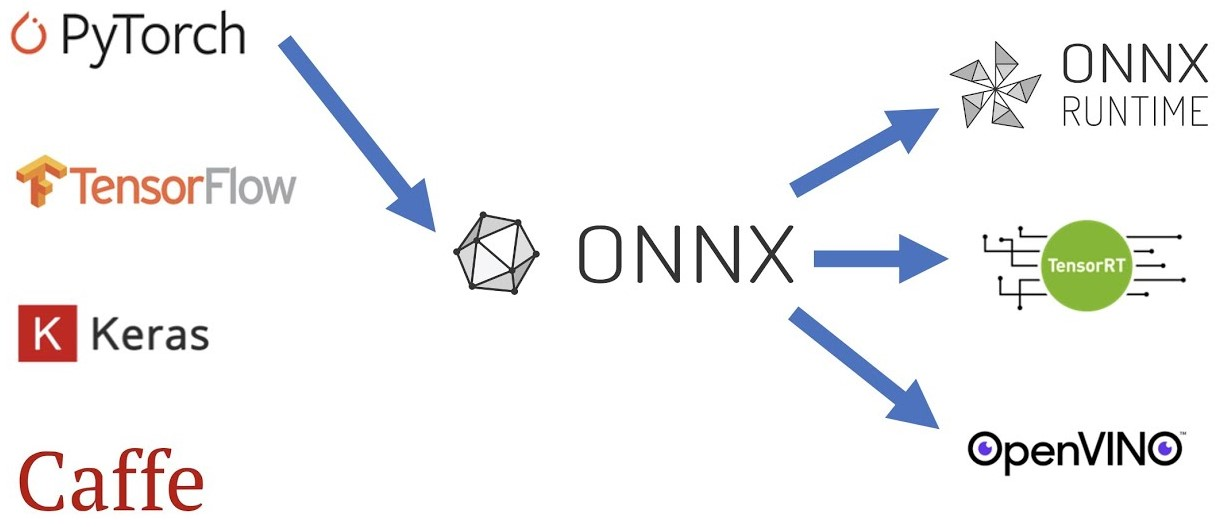
\includegraphics[scale=0.4]{gambar/pytorch-onnx-openvino.jpg}
  \caption{Flow of converting PyTorch Model to OpenVINO.}
  \label{fig:pytorch-to-openvino}
\end{figure}


\section{Choose Six Keypoints based on Humanoid Robot Keypoints}
\label{sec:choose-keypoints}

The difference in numbers between human keypoints and robot keypoints makes us have to choose certain human's keypoints in order to make a comparison between them.
Based on the results after testing, we chose Mediapipe for human and Keypoint RCNN for robot. Mediapipe provides 33 landmark keypoints for human and Keypoint RCNN only provides 6 keypoints.
Therefore, we need to choose 6 human keypoint as shown in Pseudocode \ref{lst:choose-human-keypoints}.
Note that, the name of the keypoints in the code corresponds to the name of the keypoints in the robot. First, we get all 33 keypoints. Then calculate the keypoint we want, such as the head keypoint which is located between the right and left eye.
To obtain the eye landmarks, we can index \verb|landmark| variable according to Figure \ref{fig:mediapipe-landmark}, where the left eye is index 2 and the right eye is index 5. This also applies to other landmarks.
The keypoint for the hands and feet is simply to select the wrists and ankles, where landmark[15] and landmark[16] are wrists, landmark[27] and landmark[28] are ankles.
Lastly, the trunk keypoint is located between the shoulder and hip keypoint. The x coordinate is located in the middle of the hip. The y-coordinate, on the other hand, is located on 1/4 distance between the hip and the shoulder from below.
First, we determine the midpoint between the shoulder and hip by individually calculating the coordinates of the right and left y axes, like Pseudocode \ref{lst:choose-human-keypoints} lines 19 and 21. In order to obtain 1/4 of the distance between the hip and the shoulder from below, we then compute the midpoint between the previous computation and the hip point as shown in lines 20, 22, and 24.
After all of the computation, we arrange all keypoints in a single array.

\lstinputlisting[
  language={},
  caption={Choose human keypoints.},
  label={lst:choose-human-keypoints}
]{program/choose-human-keypoints.txt}


\section{Keypoint Normalization}
\label{sec:keypoint-normalization}

When we think about the problem, we see that there are many uncertainties to be addressed. For example, human and humanoid robot can differ in height, body shape, and location within an image: one subject (human or robot) may have been nearby the camera,
while another may have been in the distance. In order to get an accurate outcome, each of these issues must be resolved.
After choosing the keypoints, the model output for both human and robot is the coordinates of 6 keypoints. This information can be used to create a new keypoint coordinates starting from (0,0) in the image. This solves the problem of the subject appearing in different parts of the picture.

\lstinputlisting[
  language={},
  caption={Get New Keypoints.},
  label={lst:new-keypoints}
  ]{program/bbox.txt}

In Pseudocode \ref{lst:new-keypoints}, the code is structured into two functions: \verb|get_min_point| and \verb|get_| \verb|new_coords|. The \verb|get_min_point| function takes an array of keypoints coordinates as input with shape (6,2)
and iterates through each item in the array. It keeps track of the minimum x and y values encountered during the iteration and returns an array containing the minimum x and y coordinates.
The \verb|get_new_coords| function takes the keypoint coordinates array and \verb|min_point| (minimum x and y coordinates) from the previous calculation as input. It iterates through each item and subtracts the corresponding minimum x and y values from each coordinate. The updated coords array is returned.

We further normalized the resulting keypoints coordinates by performing L2 normalization in order to transform it into a unit vector as shown in Figure \ref{fig:transforming-into-unit-vector}.
This means we are ignoring the size of the picture, but keeping in account the direction of the vector, created by the pose inside of that image.
To calculate the L2 normalization for an individual point is to take the square root of the sum of the squares of its coordinates. This calculation resulting the magnitude or length of the vector formed by the coordinates of the point.
Next step is dividing each coordinate by the length of the vector. This step ensures that the resulting normalized point lies on the unit circle. This normalization process scales the coordinates proportionally while preserving the direction of the vector. Moreover, it will optimize using NumPy library so it can compute multiple points simultaneously.

\begin{figure}[ht]
  \centering
  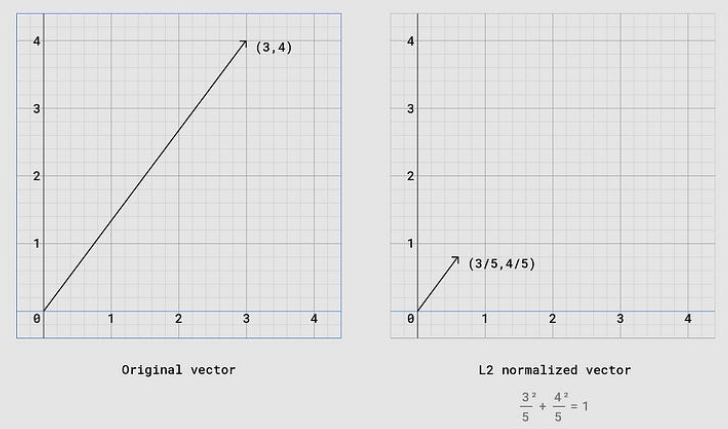
\includegraphics[scale=0.7]{gambar/transform-to-unit-vector.png}
  \caption{Transforming into Unit Vector.}
  \label{fig:transforming-into-unit-vector}
\end{figure}

\section{Comparing Human Keypoints and Robot Keypoints}
\label{sec:comparing-keypoints}

Now that we have standardized the pose vectors, it is time to choose a similarity measure. We chose cosine similarity for this particular instance, mainly because we are working with vectors and performing a few calculations detailed below to arrive at a Euclidean distance that can be interpreted as a cosine distance.
The cosine similarity ranges from -1 to 1, with 1 indicating identical poses or vectors are in the same direction, 0 indicating no similarity or vectors are nearly orthogonal, and -1 indicating completely opposite poses or opposite direction. The cosine distance, on the other hand, is a dissimilarity measure that ranges from 0 to 2.
Using Equation \ref{eq:euclideandistance} scales the values to the range of 0 to 2, making it easier to interpret the results. A larger value implies a greater dissimilarity between poses. In that equation, Fxy and Gxy are two pose vectors to be compared after L2 normalization. Moreover, Fxy and Gxy contain only x and y positions for each of the 6 keypoints, it does not include confidence scores.

\begin{equation}
  \label{eq:cosinesimilarity}
  cosineSimilarity(x,y) = \frac{x \cdot y}{|x||y|}
\end{equation}

\begin{equation}
  \label{eq:euclideandistance}
  D(F_{xy}, G_{xy}) = \sqrt{2 * (1 - cosineSimilarity(F_{xy}, G_{xy}))}
\end{equation}


\section{Pose Similarity Result}
\label{sec:pose-similarity-result}

The result of pose similarity is in percentages with a range of 0 to 100. A higher score indicates a more similar position between the human and robot, and vice versa.
In order to get it, we multiply the cosine distance result from Section \ref{sec:comparing-keypoints} by 100 and subtract the result from 100.
After getting each result of pose similarity, we take a mean and display it in the left top video. This video will be generated after detecting and comparing all poses.
\cleardoublepage

% Bab 4 pengujian dan analisis
\chapter{RESULTS AND DISCUSSION}
\label{chap:resultsandiscussion}

% Ubah bagian-bagian berikut dengan isi dari pengujian dan analisis

This section discusses and shows the results from our test and analysis on training humanoid robot model, human model comparison, and also compares their suitability.
All tests were conducted using the Ichiro robot in the \emph{Robot Cerdas} Laboratory with computer specifications as can be seen in Table \ref{tb:computerspecichiro}.

\def\arraystretch{1.5}
\begin{longtable}{|c|c|}
  \caption{Computer specification on Ichiro robot.}
  \label{tb:computerspecichiro}\\
  \hline
  OS      & Ubuntu 20.04.2 LTS \\
  \hline
  CPU     & Intel i5-10210U (8) @ 4.200GHz \\
  \hline
  GPU     & Intel UHD Graphics  \\
  \hline
  RAM     & 3636 MiB \\
  \hline
\end{longtable}


\section{New Dataset Statistics}
\label{sec:new-dataset-statistics}

This new dataset is a merge of the HumanoidRobotPose dataset and Ichiro's pose dataset. Figure \ref{fig:nimbro-statistics} shows the statistics for the HumanoidRobotPose dataset and Figure \ref{fig:new-dataset-statistics} shows the statistics for the new dataset.
The diversity of the number of robot instances per image is illustrated on the left, and the scale proportions of robot instances is shown on the right. The definition of small, medium, and large scale is identical to the COCO dataset.
Most of the additions (Ichiro's pose dataset) are one robot instance (from approximately 850 to 1700) and few are two instances per image (from approximately 380 to 430) with large scale, this was based on a system requirement that only need pose estimation for one robot.

\begin{figure}[ht]
  \centering
  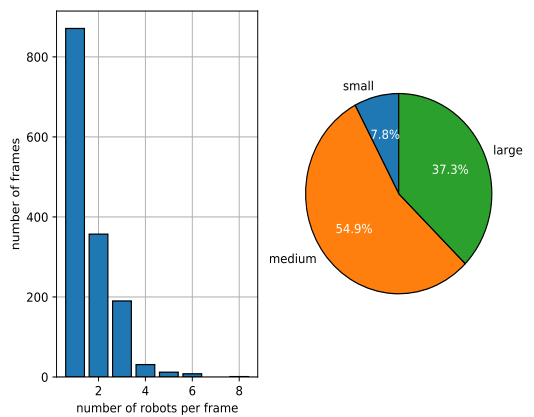
\includegraphics[scale=0.78]{gambar/old_dataset.png}
  \caption{HumanoidRobotPose Statistics.}
  \label{fig:nimbro-statistics}
\end{figure}

\begin{figure}[ht]
  \centering
  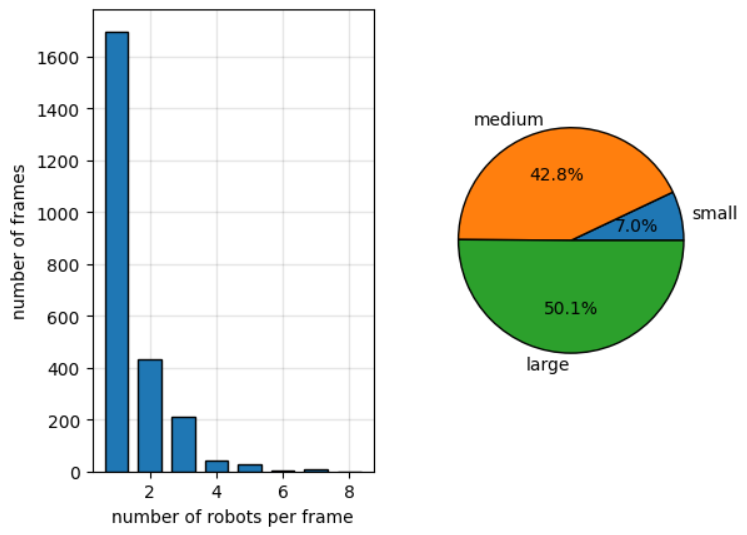
\includegraphics[scale=0.63]{gambar/new_dataset.png}
  \caption{New Dataset Statistics.}
  \label{fig:new-dataset-statistics}
\end{figure}


\section{Robot's Model Training Result}
\label{sec:robotmodeltrainingresult}

This section shows the evaluation metrics about three models and testing we perform such as visualizing detection results and inference time.
For the evaluation metrics, NimbRo's Model and Keypoint RCNN use the Object Keypoint Similarity (OKS) with a per-keypoint constant equal to 0.4 for all keypoints.
Otherwise, YOLO uses slightly different OKS, they extend the idea of IOU loss from box to keypoints. OKS is treated as IOU in case of keypoints \parencite{maji2022yolopose}.
From Table \ref{tb:robotmodelcomparison} it can be seen that Keypoint RCNN has the highest evaluation metric among the other models.
Moreover, Keypoint RCNN showed the best detection results as shown in Table \ref{tb:robotmodelcomparisondetectionresults}, followed by NimbRo's Model and YOLO-pose.
Lastly, NimbRo's Model is the most likely to be applied to real-time systems because it has the lowest inference time as shown in Table \ref{tb:inferencerobot}.
However, since our main program uses the web for interaction and during PLAY mode, there is a considerable delay due to transferring two image data from the server to the client.
Hence, we decide to store the images first and do pose comparisons afterwards. Since we are more concerned with a reliable model than a faster model, so the Keypoint RCNN model is suitable for this.

\begin{longtable}{|L{1.5cm}|c|c|c|c|c|c|c|c|c|c|}
  \caption{Robot Model Comparison.}
  \label{tb:robotmodelcomparison}\\
  \hline
  \rowcolor[HTML]{C0C0C0}
  \textbf{Model} & \textbf{AP} & \textbf{AP\textsubscript{50}} & \textbf{AP\textsubscript{75}} & \textbf{AP\textsubscript{M}} & \textbf{AP\textsubscript{L}} & \textbf{AR} & \textbf{AR\textsubscript{50}} & \textbf{AR\textsubscript{75}} & \textbf{AR\textsubscript{M}} & \textbf{AR\textsubscript{L}} \\
  \hline
  NimbRo Model & 0.828       & 0.879                         & 0.840                         & 0.886                        & 0.864                        & 0.836       & 0.884                         & 0.849                         & 0.895                        & 0.872 \\
  \hline                        
  Keypoint RCNN  & 0.879       & 0.936                         & 0.904                         & 0.859                        & 0.937                        & 0.925       & 0.973                         & 0.944                         & 0.936                        & 0.955 \\
  \hline                        
  YOLO-pose      & 0.849       & 0.838                         & -                             & -                            & -                            & 0.814       & -                             & -                             & -                            & - \\
  \hline
\end{longtable}

\def\arraystretch{0.5}
\begin{longtable}{|c|c|c|}
  \caption{Robot Model Comparison Detection Results.}
  \label{tb:robotmodelcomparisondetectionresults}\\
  \hline
  \rowcolor[HTML]{C0C0C0}
  \textbf{NimbRo's Model}    & \textbf{Keypoint RCNN} & \textbf{YOLO-pose}\\
  \hline
  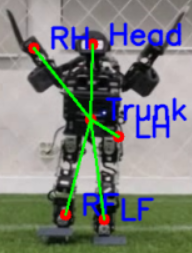
\includegraphics[scale=0.85]{gambar/nimbro-1.png} & 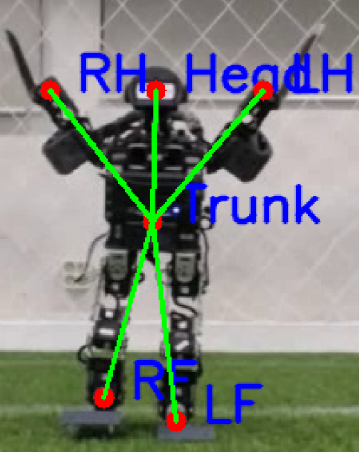
\includegraphics[scale=0.48]{gambar/rcnn-1.png} & 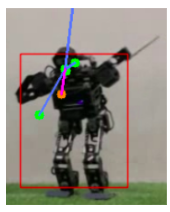
\includegraphics[scale=0.66]{gambar/yolo-1.png} \\
  \hline
  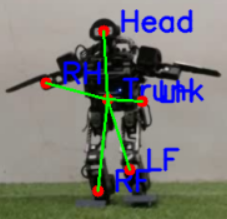
\includegraphics[scale=0.85]{gambar/nimbro-2.png} & 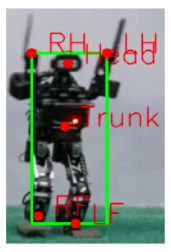
\includegraphics[scale=0.49]{gambar/rcnn-2.png} & 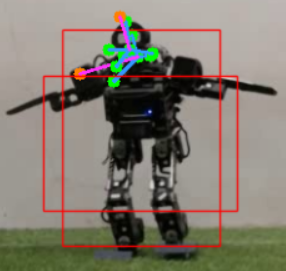
\includegraphics[scale=0.68]{gambar/yolo-2.png} \\
  \hline
  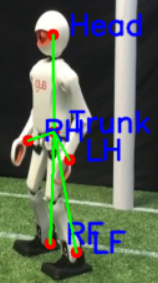
\includegraphics[scale=0.85]{gambar/nimbro-3.png} & 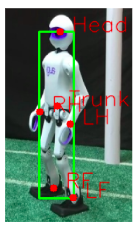
\includegraphics[scale=0.49]{gambar/rcnn-3.png} & 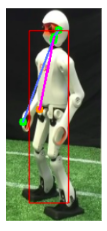
\includegraphics[scale=0.67]{gambar/yolo-3.png} \\
  \hline
\end{longtable}

\def\arraystretch{1.5}
\begin{longtable}{|c|c|c|}
  \caption{Inference Time Model Humanoid Robot.}
  \label{tb:inferencerobot}\\
  \hline
  \rowcolor[HTML]{C0C0C0}
  \textbf{Model}    & \textbf{PyTorch (s)} & \textbf{OpenVINO (s)}\\
  \hline
  NimbRo's Model & 0.4 - 0.5 & 0.15 - 0.2 \\
  \hline
  Keypoint RCNN  & 3.5 - 4.0 & 1.25 \\
  \hline
  YOLO-pose      & 0.7 - 0.75& 0.27 - 0.3 \\
  \hline
\end{longtable}


\section{Human's Model Comparison}
\label{sec:humanmodelcomparison}

Based on \parencite{bazarevsky2020} that compares three different models: BlazePose Lite, BlazePose Full, and OpenPose (body only), they test the models on AR Dataset and Yoga Dataset. As an evaluation metric, they use the Percent of Correct Points with 20\% tolerance (PCK@0.2)
(where assuming the point to be detected correctly if the 2D Euclidian error is smaller than 20\% of the corresponding person's torso size). BlazePose shows slightly worse performance than the OpenPose model on the AR dataset but BlazePose Full outperforms OpenPose on Yoga/Fitness use cases.
Note that, in this study, we use BlazePose Full because by default the value of \emph{model complexity} argument is 1 in the \emph{mediapipe.solutions.pose.Pose} API class. Mediapipe provides 3 BlazePose models: BlazePose Lite, BlazePose Full, and BlazePose Heavy. Pose landmark accuracy as well as inference latency generally go up with the model complexity.
Table \ref{tb:yoloandmediapipecomparison} shows the comparison between YOLO-pose and MediaPipe Pose and based on our needs to just detect one person, MediaPipe should be the best and also reliable choice.  

\begin{longtable}{|L{3cm}|L{5cm}|L{5cm}|}
  \caption{YOLO-pose and MediaPipe Pose Comparison.}
  \label{tb:yoloandmediapipecomparison}\\
  \hline
  \rowcolor[HTML]{C0C0C0}
  \textbf{Features}    & \textbf{YOLO-pose} & \textbf{MediaPipe Pose}\\
  \hline
  Topology             & 17 Keypoints COCO  & 33 Keypoints COCO \\
  \hline
  Workflow             & Detection runs for all frames & Detection runs once followed by tracker until occlusion occurs \\
  \hline
  GPU support          & Support for both CPU and GPU & Only CPU \\
  \hline
  Number of persons    & Multi-person & Single person \\
  \hline
\end{longtable}

\begin{longtable}{|c|c|c|}
  \caption{Inference Time Model Human.}
  \label{tb:inferencehuman}\\
  \hline
  \rowcolor[HTML]{C0C0C0}
  \textbf{Model}    & \textbf{Inference Time (s)} \\
  \hline
  Mediapipe   & 0.15 - 0.2\\
  \hline
  OpenPose    & 0.2\\
  \hline
  YOLO-Pose   & 0.7 - 0.75\\
  \hline
\end{longtable}

\section{Comparing the Suitability Between Humanoid Robot Pose and Human Pose Results}
\label{sec:comparingsuitabilityresults}

By using the method in Section \ref{sec:comparing-keypoints}, we get the result from comparing the human pose and robot pose in percentage terms.
We can see the two figures below, in Figure \ref{fig:comparingb} humans make movement that are more like robot than in Figure \ref{fig:comparinga}.
Therefore, the comparison result of Figure \ref{fig:comparingb} is higher at 91\% than Figure \ref{fig:comparinga} with just 79\%.
This indicates that the system can provide an accurate assessment between the poses of humans and robots.
Furthermore, Figure \ref{fig:comparisongtandresult} shows the comparison between ground truth and detection results using Keypoint RCNN for every robot inside the new dataset
(the left side is ground truth and the right side is detection results).

\begin{figure}
  \centering
  \begin{subfigure}[b]{0.45\textwidth}
      \centering
      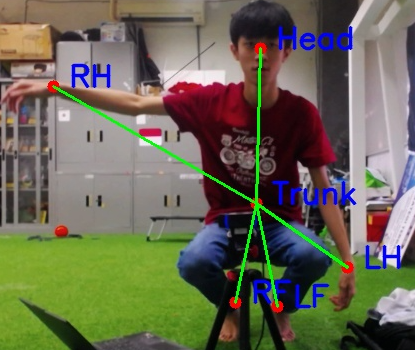
\includegraphics[width=\textwidth]{gambar/human_10_result.jpg}
      \caption{Human Image}
      \label{fig:humanimagea}
  \end{subfigure}
  \hfill
  \begin{subfigure}[b]{0.45\textwidth}
      \centering
      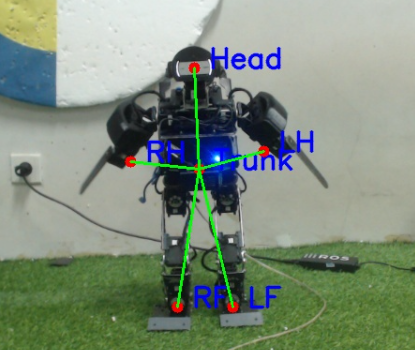
\includegraphics[width=\textwidth]{gambar/robot_6_result.jpg}
      \caption{Robot Image}
      \label{fig:robotimagea}
  \end{subfigure}
     \caption{Comparing Humanoid Robot Pose and Human Pose.}
     \label{fig:comparinga}
\end{figure}

\begin{figure}
  \centering
  \begin{subfigure}[b]{0.45\textwidth}
      \centering
      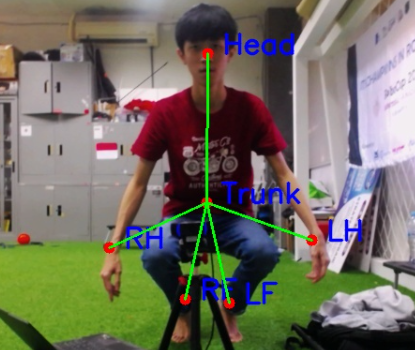
\includegraphics[width=\textwidth]{gambar/human_6_result.jpg}
      \caption{Human Image}
      \label{fig:humanimageb}
  \end{subfigure}
  \hfill
  \begin{subfigure}[b]{0.45\textwidth}
      \centering
      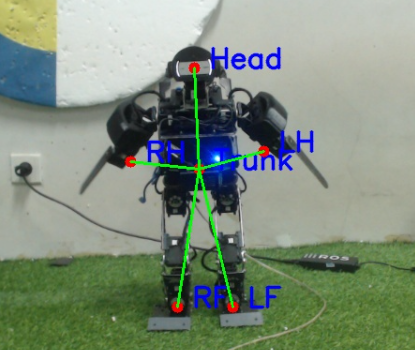
\includegraphics[width=\textwidth]{gambar/robot_6_result.jpg}
      \caption{Robot Image}
      \label{fig:robotimageb}
  \end{subfigure}
     \caption{Comparing Humanoid Robot Pose and Human Pose.}
     \label{fig:comparingb}
\end{figure}

\begin{figure}
  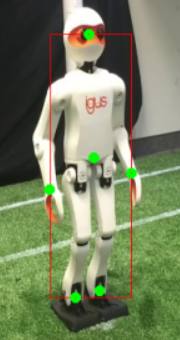
\includegraphics[width=.15\textwidth]{gambar/comp_with_gt/robot_1_gt.png}
  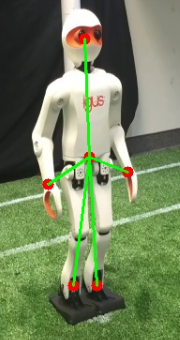
\includegraphics[width=.15\textwidth]{gambar/comp_with_gt/robot_1_res.png} \hfill%
  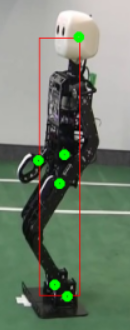
\includegraphics[width=.113\textwidth]{gambar/comp_with_gt/robot_2_gt.png}
  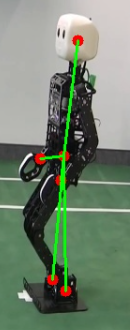
\includegraphics[width=.113\textwidth]{gambar/comp_with_gt/robot_2_res.png} \hfill%
  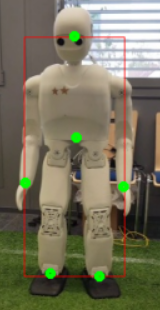
\includegraphics[width=.15\textwidth]{gambar/comp_with_gt/robot_3_gt.png}
  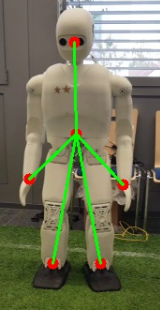
\includegraphics[width=.15\textwidth]{gambar/comp_with_gt/robot_3_res.png}
  \\[\medskipamount]
  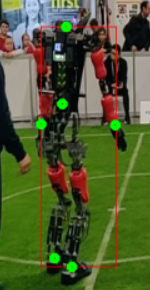
\includegraphics[width=.135\textwidth]{gambar/comp_with_gt/robot_4_gt.png}
  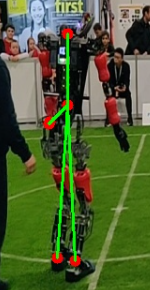
\includegraphics[width=.135\textwidth]{gambar/comp_with_gt/robot_4_res.png} \hfill%
  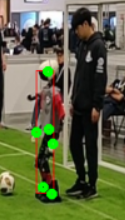
\includegraphics[width=.148\textwidth]{gambar/comp_with_gt/robot_5_gt.png}
  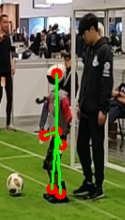
\includegraphics[width=.148\textwidth]{gambar/comp_with_gt/robot_5_res.png} \hfill%
  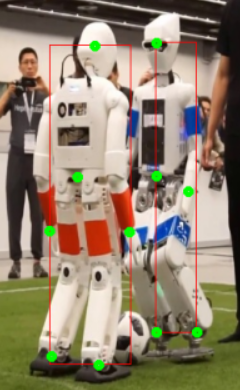
\includegraphics[width=.16\textwidth]{gambar/comp_with_gt/robot_6_gt.png}
  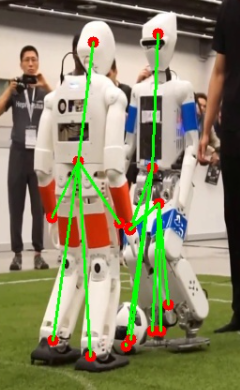
\includegraphics[width=.16\textwidth]{gambar/comp_with_gt/robot_6_res.png}
  \\[\medskipamount]
  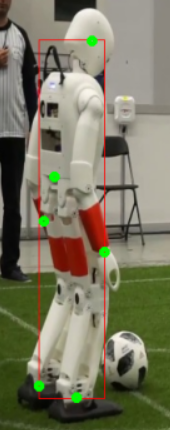
\includegraphics[width=.11\textwidth]{gambar/comp_with_gt/robot_7_gt.png}
  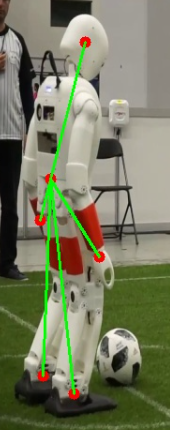
\includegraphics[width=.11\textwidth]{gambar/comp_with_gt/robot_7_res.png} \hfill%
  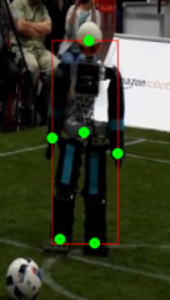
\includegraphics[width=.155\textwidth]{gambar/comp_with_gt/robot_8_gt.png}
  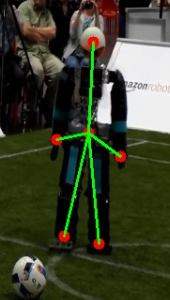
\includegraphics[width=.155\textwidth]{gambar/comp_with_gt/robot_8_res.png} \hfill%
  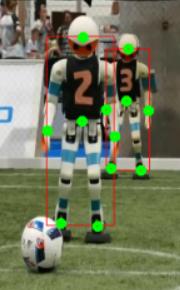
\includegraphics[width=.17\textwidth]{gambar/comp_with_gt/robot_9_gt.png}
  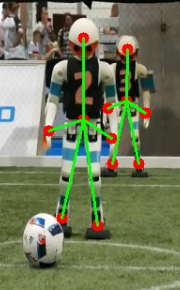
\includegraphics[width=.17\textwidth]{gambar/comp_with_gt/robot_9_res.png}
  \\[\medskipamount]
  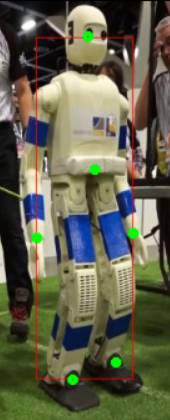
\includegraphics[width=.12\textwidth]{gambar/comp_with_gt/robot_10_gt.png}
  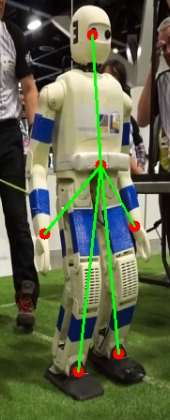
\includegraphics[width=.12\textwidth]{gambar/comp_with_gt/robot_10_res.png} \hfill%
  \includegraphics[width=.137\textwidth]{gambar/comp_with_gt/robot_11_gt.png}
  \includegraphics[width=.137\textwidth]{gambar/comp_with_gt/robot_11_res.png} \hfill%
  \includegraphics[width=.18\textwidth]{gambar/comp_with_gt/robot_12_gt.png}
  \includegraphics[width=.18\textwidth]{gambar/comp_with_gt/robot_12_res.png}
  \centering
  \captionsetup{justification=centering, margin=2cm}
  \caption{Comparison Between Ground Truth and Detection Result on Every Type of Robot in Dataset}
  \label{fig:comparisongtandresult}
\end{figure}
\cleardoublepage

% Bab 5 penutup
\chapter{PENUTUP}
\label{chap:conclusion}

Dalam bab ini, kesimpulan dari hasil pengujian akan disajikan sebagai jawaban terhadap masalah yang diangkat dalam penelitian ini.
Selain itu juga terdapat rekomendasi untuk tindakan yang dapat dilakukan dalam mengembangkan penelitian ini ke arah yang lebih lanjut.

\section{Kesimpulan}
\label{sec:summary}

Berdasarkan hasil pengujian yang telah dilakukan, penulis dapat menyimpulkan beberapa hal sebagai berikut:

\begin{enumerate}[nolistsep]

  \item RCNN Keypoint adalah metode yang mampu untuk mendeteksi pose robot \textit{humanoid} dengan 6 \textit{keypoint} karena mengungguli model lain,
        dengan hasil AP sebesar 0.879 dan AR sebesar 0.925 pada test set (kecuali untuk AP \textit{medium}).
  \item Kesamaan Kosinus merupakan metode yang cocok untuk membandingkan pose robot dan manusia karena hasilnya akan lebih tinggi
        ketika manusia melakukan gerakan yang lebih menyerupai gerakan robot dan hasilnya akan lebih rendah ketika gerakan manusia tidak semirip dengan gerakan robot.

\end{enumerate}

\section{Saran}
\label{chap:suggestionsandfuturework}

Untuk pengembangan lebih lanjut pada penelitian mendatang, maka penulis memiliki saran sebagai berikut:

\begin{enumerate}[nolistsep]

  \item Menambahkan robot \textit{humanoid} dengan ukuran \textit{teen} ke dalam dataset sehingga tipe dari robot tanpa kulit dapat lebih beragam.
  \item Mencoba menambah \textit{keypoint} pada robot \textit{humanoid} sehingga hasil perbandingan pose lebih akurat.

\end{enumerate}

\cleardoublepage

\chapter*{DAFTAR PUSTAKA}
\addcontentsline{toc}{chapter}{DAFTAR PUSTAKA}
\renewcommand\refname{}
\vspace{2ex}
\renewcommand{\bibname}{}
\begingroup
\def\chapter*#1{}
\printbibliography
\endgroup
\cleardoublepage

% Biografi penulis
\begin{center}
  \Large
  \textbf{BIOGRAFI PENULIS}
\end{center}

\addcontentsline{toc}{chapter}{BIOGRAFI PENULIS}

\vspace{2ex}

\begin{wrapfigure}{L}{0.3\textwidth}
  \centering
  \vspace{-3ex}
  % Ubah file gambar berikut dengan file foto dari mahasiswa
  \includegraphics[width=0.3\textwidth]{gambar/nathan.jpg}
  \vspace{-4ex}
\end{wrapfigure}

Penulis bernama \name{} yang akrab disapa Nathan, lahir pada tanggal 24 August 2001 di kota Surabaya, Jawa Timur.
Penulis telah menempuh pendidikan di SD Katolik Sang Timur Pasuruan lulus pada tahun 2013, SMP Katolik Sang Timur Pasuruan lulus pada tahun 2016, dan SMA Katolik St. Louis 1 Surabaya lulus pada tahun 2019.
Penulis kemudian melanjutkan pendidikan sarjana di Departemen Teknik Komputer Institut Teknologi Sepuluh Nopember melalui jalur SBMPTN pada tahun 2019.
Selama aktif menjadi mahasiswa, penulis telah bergabung ke dalam dalam Tim Robotika Ichiro sebagai \textit{programmer} dan Asisten Laboratorium B401.
Sebagai bagian dari Tim Ichiro, penulis telah meraih beberapa prestasi nasional dan internasional seperti Kontes Robot Indonesia Nasional 2020 dan 2021, FIRA SimulCup 2021 dan 2022 yang diselenggarakan secara daring,
serta Kontes Robot Indonesia Nasional 2022 dan RoboCup 2022 Bangkok yang diselenggarakan secara luring
Penulis juga telah bergabung dengan Bangkit Academy 2022 pada jalur \textit{Machine Learning} dan memiliki pengalaman magang selama 3 bulan di PT Indosat Tbk untuk menyelesaikan Program Bangkit Academy.
Minat penulis dalam mengerjakan tugas akhir adalah \textit{Machine Learning} dan \textit{Computer Vision}. Penulis dapat dihubungi melalui email nathanael.hutama24@gmail.com.
\cleardoublepage

\end{document}
